\chapter{Introduction}
\label{ch:Intro}


%%%%%%%%%%%%%%%%%%%%%%%%%%%%%%%%%%%%%%%%%%%%%%%%%%

In this thesis I have use a functional genomics approach to characterise the regulatory landscape in psoriasis and psoriatic arthritis, with the aim of uncovering the mechanism of action of disease risk variants. In this chapter, I begin by reviewing the current knowledge of disease pathophysiology, the role of genetic variation, and then describe cutting edge functional genomics approaches in complex disease research that are relevant to the subsequent chapters.

\section{Psoriasis and psoriatic arthritis}
%
Psoriasis and psoriatic arthritis (PsA) have been described as two distinct common complex disease entities that share nonetheless certain clinical features and genetic architecture. Psoriasis is a chronic inflammatory dermatose disease with episodes of relapse and remittance \parencite{Nestle2009}. On the other hand, PsA is a seronegative chronic inflammatory disease within the spondyloarthritis family that usually develops after psoriasis skin manifestations\parencite{Moll1973, Coates2016, Villanova2016}. The study of similarities and differences between the conditions at the pathological and genetic levels will benefit the understanding of genetic variability in the risk of developing psoriasis and PsA as well as the identification of new therapeutic targets.

%(Variants in RUNX3 contribute to susceptibility to PsA, exhibiting further common ground with ankylosing spondylitis, PsA Immunochip)

\subsection{Epidemiology and global impact}
%
Psoriasis represents a serious global health problem that currently affects about 100 million people worldwide, including both children and adults with no sex bias \parencite{Organization2016}. Onset of disease seems to have a bimodal distribution with psoriasis patients being classified as early-onset/ type I (around 16-22 and 30-39 years) or late-onset / type II (between 50-60 years) \parencite{Henseler1985}. This classification based on the age of onset also has correlates with distinctive clinical features including severity, relapse frequency and family history. As reflected in the minor correlation with geographic latitude, the risk of developing psoriasis has a strong ethnicity component \parencite{Jacobson2011}. In fact, the prevalence of psoriasis in adults is lower among African, African American and Asian (between 0.4 and 0.7\%) compared to American and Canadian populations (4.6 and 4.7\%, respectively). 

In the UK, psoriasis prevalence ranges between 2 and 3\%, affecting approximately 1.8 million people \parencite{Perera2012}. On the other hand, cases of PsA in the general population varies between 0.04 and 1.2\% \parencite{Perera2012} but dramatically increase up to 10 to 30\% within psoriasis patients, evidencing the strong association between the two diseases \parencite{Gelfand2005,Reich2008}. In the UK, 14\% of psoriasis patients develop chronic inflammatory arthritis in the form of PsA during the course of the disease \parencite{Ibrahim2009}. Overall, data suggest an steady increase in both psoriasis and PsA prevalence over time \parencite{Springate2007,Organization2016}. 

Several comorbidities have also been associated with psoriasis and PsA, with comparatively greater prevalence in PsA. For example, intraocular inflammation known as uveitis affects 8\% of PsA patients compared to only 2\% of psoriasis patients \parencite{Husted2011, Oliveira2015}. Other comorbidities include IBD, cardiovascular disease (CVD), type II diabetes (T2D) and metabolic syndrome \parencite{ Gelfand2006, Shapiro2007,Cohrn20017}. Psoriasis and PsA have also been associated with an increased prevalence of depression and suicidal ideation \parencite{Sampogna2012}. Accordingly, psoriasis and PsA represent a burden for the economy due to treatment costs and associated morbidity. In the UK treatment and management-associated costs for psoriasis in 2015 accounted for \textsterling4,000 to \textsterling14,000, before and after requirements of biological therapy, respectively \parencite{Burgos-Pol2016, Poole2010} and the costs are further enhanced in the case of PsA.





\subsection{Psoriasis and inflammatory dermatoses}
%

The skin is the biggest organ in the human body constituting an effective barrier between the environment and the internal organs. The most external layer, the epidermis, plays an important role in innate and adaptive immunity and its alterations, due to exogenous or endogenous factors, can lead to development of inflammatory dermatose conditions, such as psoriasis or atopic dermatitis (AD) \parencite{Johnson-Huang2009, Proksch2008}}. The group of inflammatory dermatoses affects up to 70\% of the UK population and represents the 4$^{th}$ leading cause of nonfatal burden \parencite{ICD-10,Roderick2014}. 

Lesions in psoriasis are very heterogeneous in type (pustular and non-pustular), location and severity, which complicates its clinical classification \parencite{Perera2012}. As a result, several phenotypes including psoriasis vulgaris, guttate, pustular, erythroderma and nail pitting have been defined \parencite{Marrakchi2011}.



\subsection{PsA and spondyloarthropathies}
%
PsA belongs to the family known as spondylarthropathies (SpA), which includes phenotypes such as ankylosing spondylitis (AS), reactive arthritis (ReA), idiopathic inflammatory bowel disease (IBD) and undifferentiated SpA \parencite{Baeten2013}. All these SpA subtypes are characterised by structural damage (bone formation and erosion) as well as inflammation of joints and extra-articular sites such as eyes, gut and skin. Broadly, SpA has been classified into axial and peripheral based on the affected joints (spine/sacroilicac or peripheral) and the presence of extra-articular features \parencite{Runwaleit2001, Runwaleit2001}. Studies in human families and rat models with HLA-B27 positive status have shown manifestation of different SpA forms, such as psoriasis and inflammatory bowel disease (IBD), within a single family or individual \parencite{Hammer1990,Said-Nahal2000}. These observations support the hypothesis that SpA subtypes may in fact be a single multifaceted condition with shared genetic, immunophatological and structural features and dynamic phenotypes \parencite{Baeten2013}. Conversely, some studies suggest that the immunopathological differences between axial and peripheral arthritis could be partially explained by genetic factors \parencite{Porcher2005, Appel2011, Noordenbos2012}.

As a phenotype, PsA can be further subdivided in five clinical groups as per the Moll and Wright criteria: distal, destructive, symmetric, asymmetric and spinal \parencite{Moll1973}. These subclasses mainly differ in the location, number and distribution of the affected joints and have been later modified to also include dactylitis (diffuse swelling of a digit), a distinctive feature of PsA \parencite{Reich2009}. Overall, this phenotypic heterogeneity of PsA increases the difficulty in the design and achievement of meaningful outcomes from clinical studies.




\section{Pathophysiology of psoriasis and psoriatic arthritis}

\subsection{Clinical presentation and diagnosis}
%
Of the aforementioned phenotypes, approximately 90\% of all psoriasis cases are psoriasis vulgaris, which manifests with well demarcated plaques, erythema and scaling. Plaque formation is the result of thickening (acanthosis) and vascularisation of the epidermis and can vary in size and distribution, with the most common locations being the elbows, knees and scalp \parencite{ Perera2012,Griffiths2007}. The second most common clinical presentation is psoriasis guttate (10\% of all cases) characterised by acute onset of small droplike papules usually in the trunk and proximal extremities \parencite{Vence2015}. Despite psoriasis vulgaris and guttate representing an important burden for patient wellbeing, they are not life-threatening forms of disease. Conversely, the least prevalent phenotype, pustular psoriasis has a 50\% increased risk of mortality compared to the milder psoriasis phenotypes \parencite{Gelfand2007,Moura2015}.  

As mentioned above, in addition to the difference in time of onset, type I and type II psoriasis also differ in clinical presentation. Type I psoriasis patients, with greater prevalence of HLA-C*06:02 (85.4\% of the cases) and stronger family history, commonly present guttate lesions followed very often by bacterial infection, particularly \textit{Streptococcus} throat infection \parencite{}. In contrast, type II psoriasis, where individuals are positive for HLA-C*06:02 only in 14.6\% of the cases, involves spontaneous chronic plaques such as psoriasis vulgaris \parencite{Perera2012}. 


In the case of PsA, symmetric/polyarticular PsA constitutes the most common manifestation (more than 50\% of the cases) followed by asymmetric/oligoarticular PsA (around 30\%), which exclusively affects single or few distal interphalangeal or phalangeal joints \parencite{Reich2009, McGonagle2011}. Skin psoriatic lesions precede joint inflammation in approximately 60 to70\% of the cases \parencite{Gladman2005, McGonagle2011}. In particular, nail pitting and scalp and intergluteal skin lesions constitute a predictive biomarker for development of joint inflammation \parencite{Moll1976,Griffiths2007,McGonagle,2011}. This observation reinforces the need for appropriate coordination between dermatologists and rheumatologists for an early diagnosis and treatment that could prevent functional joint disability.

The diagnosis of psoriasis and PsA is primarily based on clinical assessment of the patient`s symptoms due to the lack of appropriate molecular biomarkers at early stages of the disease \parencite{Villanova2013}. The evaluation of skin lesion severity poses an additional challenge, and different measures have been implemented for criteria unification. The Psoriasis Area and Severity Index (PASI) is the most widely quantitative rating score of skin lesion severity in research and clinical trials \parencite{Fredriksson1978,Finlay2005}. PASI quantifies the lesional burden weighted by body part based on area of affected surface and the degree of erythema’s severity, induration and scale at each location (Table \ref{tab:PASI}). Disease is considered mild for PASI scores below 7 and is classified as moderate-to-severe for PASI scores between 7 to 12, depending on the study \parencite{Finlay2005, Schmitt2005,Langewouters2008}.


\begin{table}[htbp]
\setlength{\tabcolsep}{20pt}
\renewcommand{\arraystretch}{1.5}
\begin{tabular}{@{} c c}
\toprule
\textbf{PASI} & \textbf{Description} \\
\midrule
\midrule
Body location  & Head and neck, upper limbs, trunk and lower limbs\\
Feature        & Redness, thickness and scaling \\
Severity scale & Absent, mild, moderate, severe or very severe \\
Affected area (\%)  & 0, 1-9, 10-29, 30-49, 50-69, 70-89 or 90-100 \\
\bottomrule
\end{tabular}
\medskip %gap
\caption[Variables and scoring used in the Psoriasis Area and Severity Index (PASI)]{\textbf{For each of the four body locations the test quantifies the percentage of affected area and the severity of three intensity features: redness, thickness and scaling. The score ranges from 0 (no disease) to 72 (maximal disease).}}
\label{tab:PASI}
\end{table}
\bigskip %bigger space


To diagnose PsA, modified Moll and Wright criteria known as Classification Criteria for Psoriatic Arthritis (CASPAR) are most widely used in a clinical setting \parencite {Taylor2006}. A positive diagnosis based on CASPAR requires display of inflammatory arthritis, enthesitis, and/or spondylitis and three points from a list of associated elements. In terms of disease activity and treatment efficacy, the PsA Response Criteria (PsARC) is the preferred measure \parencite{Philipp2011,Clegg1996}. PsARC considers the number of tender joints (TJC) and swollen joints (SJC) over 68 and 66, respectively, as well as patient and physician global assessment of the individual's general health based on a short questionnaire (Table \ref{tab:PsARC}). 

\begin{table}[htbp]
\setlength{\tabcolsep}{20pt}
\renewcommand{\arraystretch}{1.5}
\begin{tabular}{@{} c c}
\toprule
\textbf{PsARC} & \textbf{Description} \\
\midrule
\midrule
TJC  & Number of tender joints over 68\\
SJC  & Number of swollen joints over 66 \\
Patient’s global health assessment  & Evaluation of the patient's health\\
                                    & by the patient (scale 0 to 5)\\
Physician global health assessment  & Evaluation of the of the patient's \\
                                    & by the physician (scale 0 to 5) \\
\bottomrule
\end{tabular}
\medskip %gap
\caption[Variables and scoring used in the Psoriatic Arthritis Response Criteria (PsARC)]{\textbf{Variables and scoring used in the Psoriatic Arthritis Response Criteria (PsARC).} The patient's global health assessment by the patient and the physician is scored using a 5-point Likert scale, where 0 corresponds to very good, no symptoms and 5 corresponds to very poor and severe symptoms. When used to evaluate overall improvement after 12 weeks of treatment, improvement in at least two of the four variables evaluated (one of which must be TJC or SJC score) with no worsening of any criteria is required.}
\label{tab:PsARC}
\end{table}
\bigskip %bigger space



%\begin{landscape}
%\begin{table}[ht]
%\renewcommand{\arraystretch}{1.5}
%\begin{tabular}{cccccccc}
		%\multicolumn{2}{}{\textbf{CASPAR: a patient must have inflammatory articular disease (joint, spine, or enthesial) }} \\
		%\multicolumn{2}{}{\textbf{ with three points from five categories}} \\
		%\midrule
		%\midrule
    %\multirow{3}{*}{Psoriasis} & a. Current skin or scalp disease \\ & b. History of psoriasis \\ & c. Family history of psoriasis \\
    %\hline
		%\multirow{1}{*}{Psoriatic nail involvement} & Typical psoriatic nail distrophy\\ 
		%\hline
    %\multirow{1}{*}{A negative test for RF} & Using preferrably by enzyme-linked immunosorbent assay (EMSA)\\ 
    %\hline
    %\multirow{2}{*}{Dactylitis} & a. Swelling of an entire finger \\ & b. History of dactylitis\\ 
    %\hline
		%\multirow{1}{*}{Radiologic evidence of juxtaarticular new bone formation} & Ossification near joint margins\\ 
		%\hline
    %\bottomrule
		%\end{tabular}
		%\medskip %gap
		%\caption[CASPAR criteria for diagnosis of PsA]{\textbf{xxxx}}
%\label{tab:CASPAR}
%\end{table}
%\end{landscape}
%\bigskip %bigger space


%PsARC is composed of four measures,including: 1) patient global assessment of disease activity (improvement of 1 on a 5 point Likert scale is required for a response), 2) physician global assessment of disease activity (improvement of 1 on a 5 point Likert scale is required for  esponse), 3) joint pain (reduction of 30% or more in total score, assessing either 68 or 78 joints, using a 4 point scale is required for a response), and 4) joint swelling (reduction of 30% or more in total score, assessing either 66 or 76 joints using a 4 point scoring scale, is required for a response).




\subsection{Aetiology of psoriasis and PsA}

Psoriasis and PsA are complex chronic inflammatory diseases characterised by a dysregulated immune response initiated as the result of genetic predisposition and exposure to particular environmental cues (Figure\ref{fig:PSO_aetiology_diagram}). The origin of both pathologies, as well as the connection between skin and joint inflammation, still remain controversial. In the specific case of psoriasis, it also unclear whether disruption of the skin triggers activation of the immune response or vice versa.

%\begin{figure}[H]
%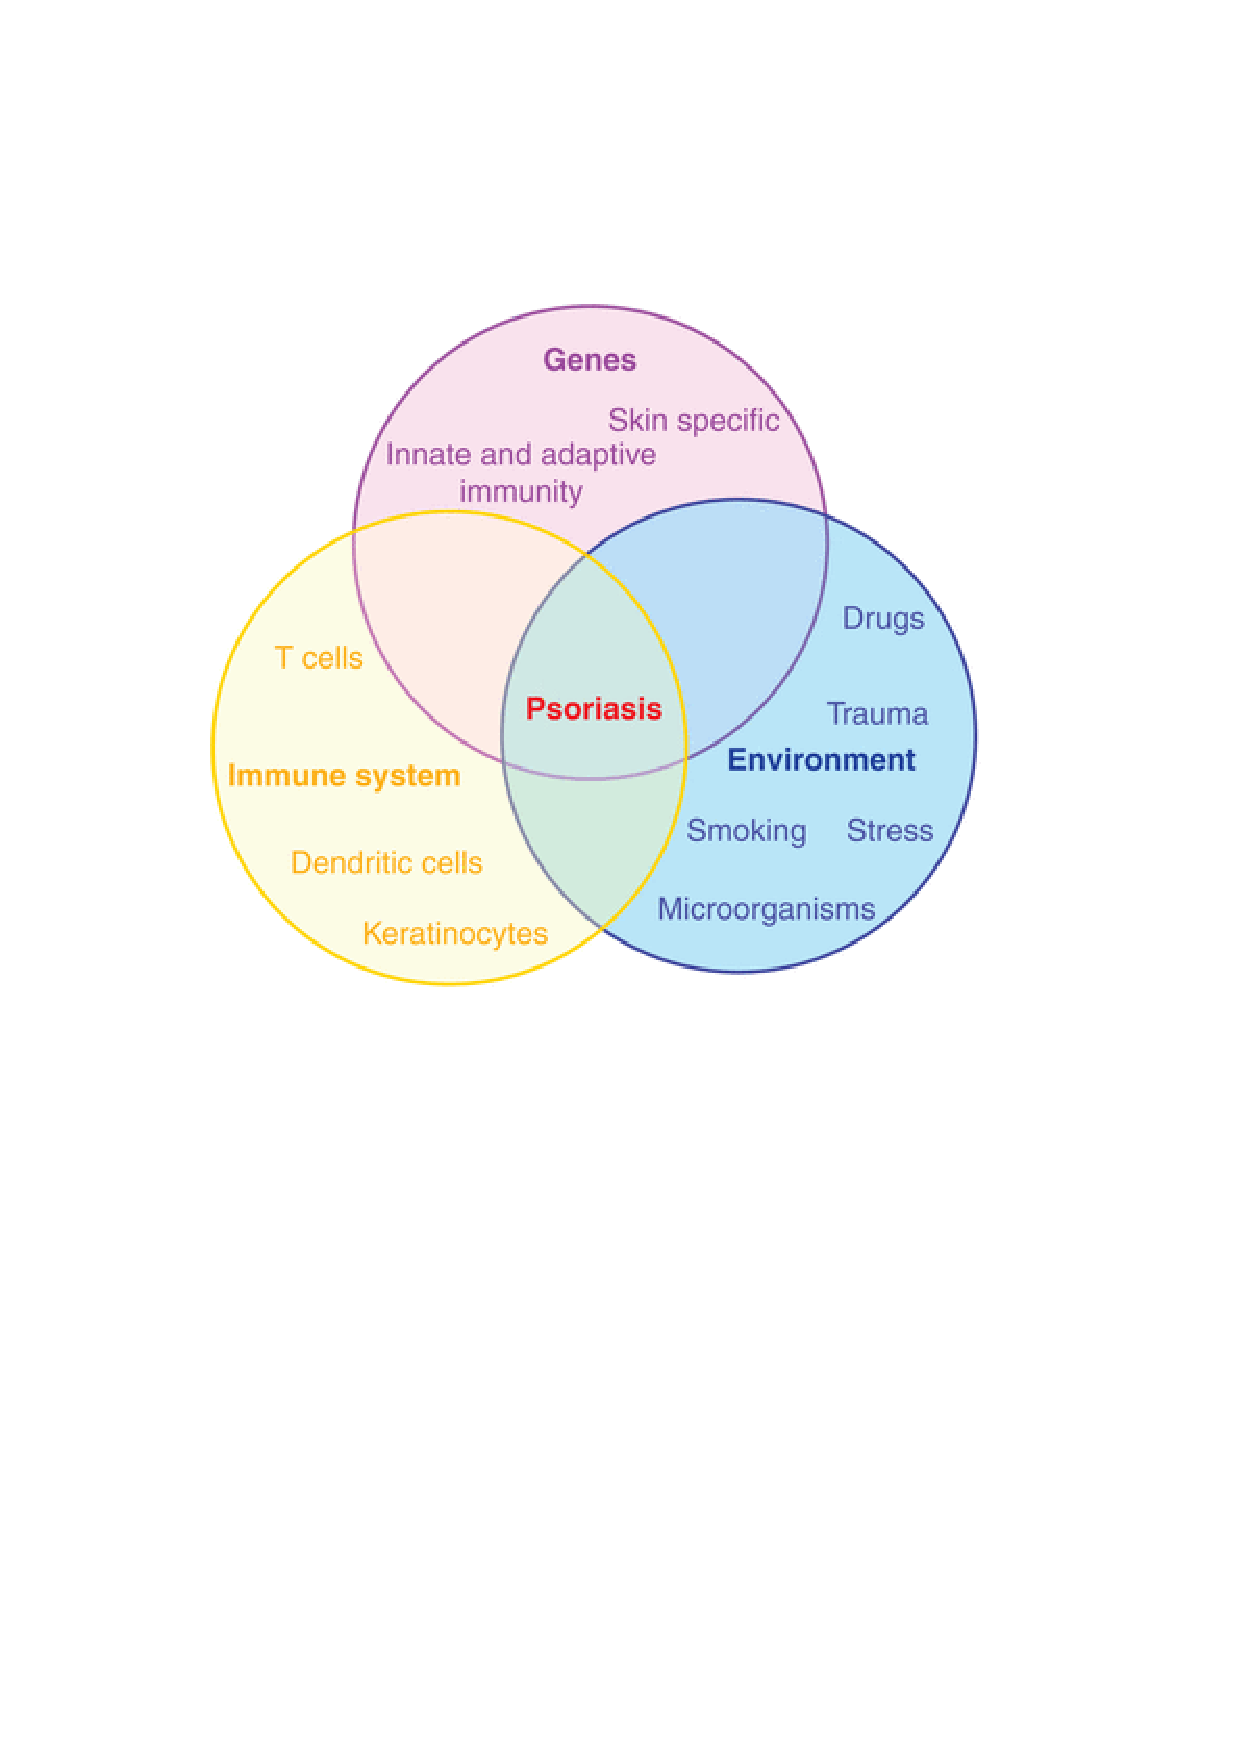
\includegraphics[width=\textwidth]{./Introduction/pdfs/PSO_aetiology_diagram_Di_Meglio_et_al_2014.pdf}
%\caption[Main factors involved in psoriasis disease aetiology]{\textbf{Figure adapted from \parencite{Meglio2014}}}
%\label{fig:PSO_aetiology_diagram}
%\end{figure}

\subsubsection*{Environmental factors and disease}
Several environmental factors are known to be associated with increased risk of development and worsening of psoriasis and PsA. A wide range of drugs including antidepressant, antihypertensive and anticytokine therapies have been clinically associated with initiation, exacerbation and worsening of psoriasis \parencite{Kim2010}. Bacterial agents such streptococcal throat infection have also been associated with development of type I psoriasis \parencite{Gudjonsson2003,Valdimarsson2009, Diluvio2006}. Consistent with other chronic inflammatory diseases such as IBD and AS, recent studies have also observed perturbation in the composition of the gut and skin microbiota of psoriasis and PsA patients \parencite{add reference}. Furthermore, physical traumaand mechanical stress can trigger the appearance of skin lesions and digit joint inflammation \parencite {Weiss2002,Nestle2009}. Lastly, behavioral factors including smoking, alcohol and stress have been linked to psoriasis and PsA but no clear association with disease development has been established yet \parencite{Meglio2014}.


\subsubsection*{Histopathological alterations in skin and joints}

The epidermis is the most external compartment of the skin, formed by approximately 90\% keratinocytes (KCs) and organised in a layer-like structure that self-renews in an spatial and time-dependent manner \parencite{Wikramanayake2014}. KC differentiation is associated with changes in morphology, replication ability and keratin composition of the intracellular matrix. In the context of psoriasis, impaired epidermis cell renewal leads to histological alterations and lesion development. Importantly, KCs undergo upregulation in the proliferation rate (hyperplasia) that causes aberrant cell differentiation (parakeratosis), thickening of the epidermis and subsequent scale formation (Ruchusatsawat2011). Concomitantly, inflammation causes immune cell infiltration and hypervascularisation of the lesion driven by upregulation in the expression of angiogenic factors and activation of the endothelium \parencite{Perera2012}.  

% Check content accuracy
In PsA, the joint affection, arising after skin lesions in the majority of the cases, involves a wide range of histological changes \parencite{Haddad2013}. One of the most common structural changes is arthritis caused by the swelling and inflammation of the joints \parencite{Schett2011}. As a result of this inflammation, alterations in bone remodeling lead to osteolysis with subsequent bone resorption and erosion at the affected joints \parencite{Mensah2017}. Bone erosion is also the main histopathological process driving dactylatis, where bone lysis resolves in shortening of the digits \parencite{Gladman2005}. Moreover, 35\% of PsA patients also undergo inflammation of the connective tissue at the insertion of tendons or ligaments, a phenomenon known as enthesitis \parencite{McGonagle2011,Polachek2017}. The inflammatory environment at the entheses favours bony spurs formation along the insertion sites, alike in RA, causing structural debilitation of the joints parencite{Benjamin2009,Finzel2014}.

 
%https://onlinelibrary.wiley.com/doi/full/10.1002/art.38794
%Schett2011


\subsubsection*{Dysregulation of the innate and adaptive immune response}
%link to the histological changes
The dysregulated immune response in psoriasis and PsA is the result of the interaction between innate and adaptive immune cells through feedback loops and a complex cytokine milieu. 

Interferon (IFN)-$\alpha$ and $\gamma$ are amongst the most relevant innate immune cytokines involved in disease initiation \parencite{Leanne2009}. Both cytokines are mainly produced by circulating plasmacytoid dendritic cells (pDCs) and myeloid DC (mDCs), respectively, upon activation by KCs pro-inflammatory cytokines \parencite{Perera2012}. Increased mRNA levels for both INFs have been detected in lesional skin and demonstrated to contribute to lymphocyte recruitment and maintenance of DCs activation \parencite{Schmid1994}. TNF-$\alpha$ is another pivotal cytokine involved in the psoriasis and PsA dysregulated innate immune. TNF-$\alpha$ is produced by activated KCs, mast cells, NK
%include NK reference
 and also adaptive immune cell types, including T helper (Th)-1 and Th-17 lymphocytes infiltrated in the skin lesions and inflamed joints \parencite{Perera2012,Lizzul2005}. This cytokine causes activation of the nuclear factor kappa-light-chain-enhancer of activated B cells (NF-$\kappa$B), a master transcriptional regulator of both, the innate and adaptive immune system that induces expression of pro-inflammatory cytokines, antiapoptotic genes and genes involved in chronic inflammation maintenance \parencite{Lizzul2005, Johansen2010}. Moreover, TNF-$\alpha$ has a prominent role in bone turnover and bone remodeling, key features of the histopathological PsA joint alterations\parencite{Mensah2008}. 
 % Johansen 2010 Preferential inhibition of the mRNA expression of p38 mitogen-activated protein kinase regulated cytokines in psoriatic skin by anti-TNF-a therapy. 

Interleukin-23 (IL-23) and interleukine-17 (IL-17) constitute a link between the innate and adaptive immunity as well as a key loop for the perpetuation of the psoriasis and PsA inflammatory response. IL-23 is an innate immune cytokine mainly produced by the mDCs and macrophages homing the inflamed skin (ref). IL-23 exerts its function through binding to the IL-23 receptor (IL-23R), highly expressed by the lesion resident DCs and T cells and the circulating CD4$^$ lymphocytes (ref). In psoriasis, IL-23 mediates the pathogenic loop between activated KCs and T cells (ref). The activation of the IL-23 pathway importantly leads to increased IL-17 cytokine levels as a result of NF-$\kapa$B activation %by \textit{TRAF3IP2} (ref). IL-17 maintains the perpetuation of the Th-17 immune mediated response through recruitment and activation of neutrophils, induction of pro-inflammatory cytokines, including interleukine-1$\beta$ (IL-1$\beta$) and interleukine-6 (IL-6), and sustains KCs activation (ref) (https://www.ncbi.nlm.nih.gov/pmc/articles/PMC3580541/). % add info
More recently, interleukin 22 (IL-22) has gained relevance as mediator of the dysregulated crosstalk between the innate and adaptive immune response. IL-22 levels are increased in the skin lesions and the serum of psoriatic patients and is mainly produced by a subset of CD4$^+$ cells known as Th-22 (ref). IL-22 contributes to some of the histological changes in skin as well as to AMP production by KCs (ref).

% Maybe a paragraph to connect skin and joint affection Identical T cell clonality between skin and synovium https://ac.els-cdn.com/S0198885999000348/1-s2.0-S0198885999000348-main.pdf?_tid=5efa7316-fde5-11e7-8091-00000aacb360&acdnat=1516454913_dd20efb867f822d68d8b09873601e8ad


\subsection{Cell types involved in psoriasis and PsA pathogenesis}
%Global report on psoriasis, 2016

Psoriasis and PsA are complex dynamic pathophysiological processes, and the understanding of the relative importance of different cell types at different disease stages still remains challenging.

Several studies have shown the role of KCs as immune sentinels through MHC-II antigen presentation and production of antimicrobial peptides (AMP), cytokines and chemokines \parencite{Black2007}. Indeed, complex formation between the cationic AMP LL-37 and self-DNA/RNA released by KCs has been observed upon damage triggered by environmental factors \parencite{Lande2007}. This complex acts as an antigen for activation of the skin-resident DCs that initiate and perpetuate the skin inflammatory response through secretion of pro-inflammatory cytokines, including IL-1, IL-6 and TNF-$\alpha$ \parencite{Feldmeyer2007, Arend2008, Nestle2009, Nestle2005}. Furthermore, \textit{in vivo} studies have described the development of psoriatic lesions in immunodeficient mice upon human xenotransplant of psoriatic skin\parencite{Boyman2004}. Altogether, these findings support the role of epidermis dysfunction in the initiation of the psoriatic chronic inflammatory response \parencite{Proskch2008}.  The relevance of KCs at early stages of psoriasis pathogenesis is reinforced by the genetic association between KC-specific genes from the late cornified envelope (LCE) family and increased psoriasis risk \parencite{Tsoi2012}

mDCs and pDCs are also considered important innate immune cells in disease initiation through antigen presentation, T-cell activation and the subsequent adaptive immune response\parencite{Mahil20016}. pDCs are circulating professional antigen presentation cells (APCs) that only upon activation by the KCs self-DNA-LL-37 complex infiltrate into the lesional and uninvolved dermis of psoriasis patients \parencite{Nestle2005, Lande2007}. In contrast, quiescent mDCs are epidermal resident cells that undergo maturation in presence of the IFN-$\alpha$ secreted by pDCs, expanding up to 30-fold only in the lesional skin \parencite{Zaba2007}. The activated mDCs mediate the Th-1 and Th-17 response as well as perpetuation of KC activation through IL-23 production (ref). Studies in immunodeficient psoriasis mouse models have shown that blockage of downstream IFN-$\alpha$ signaling or IFN-$\alpha$ production by pDCs failed to induce T-cell activation and psoriasis onset \parencite{Nestle2005}. 


\begin{figure}[htbp]
\centering
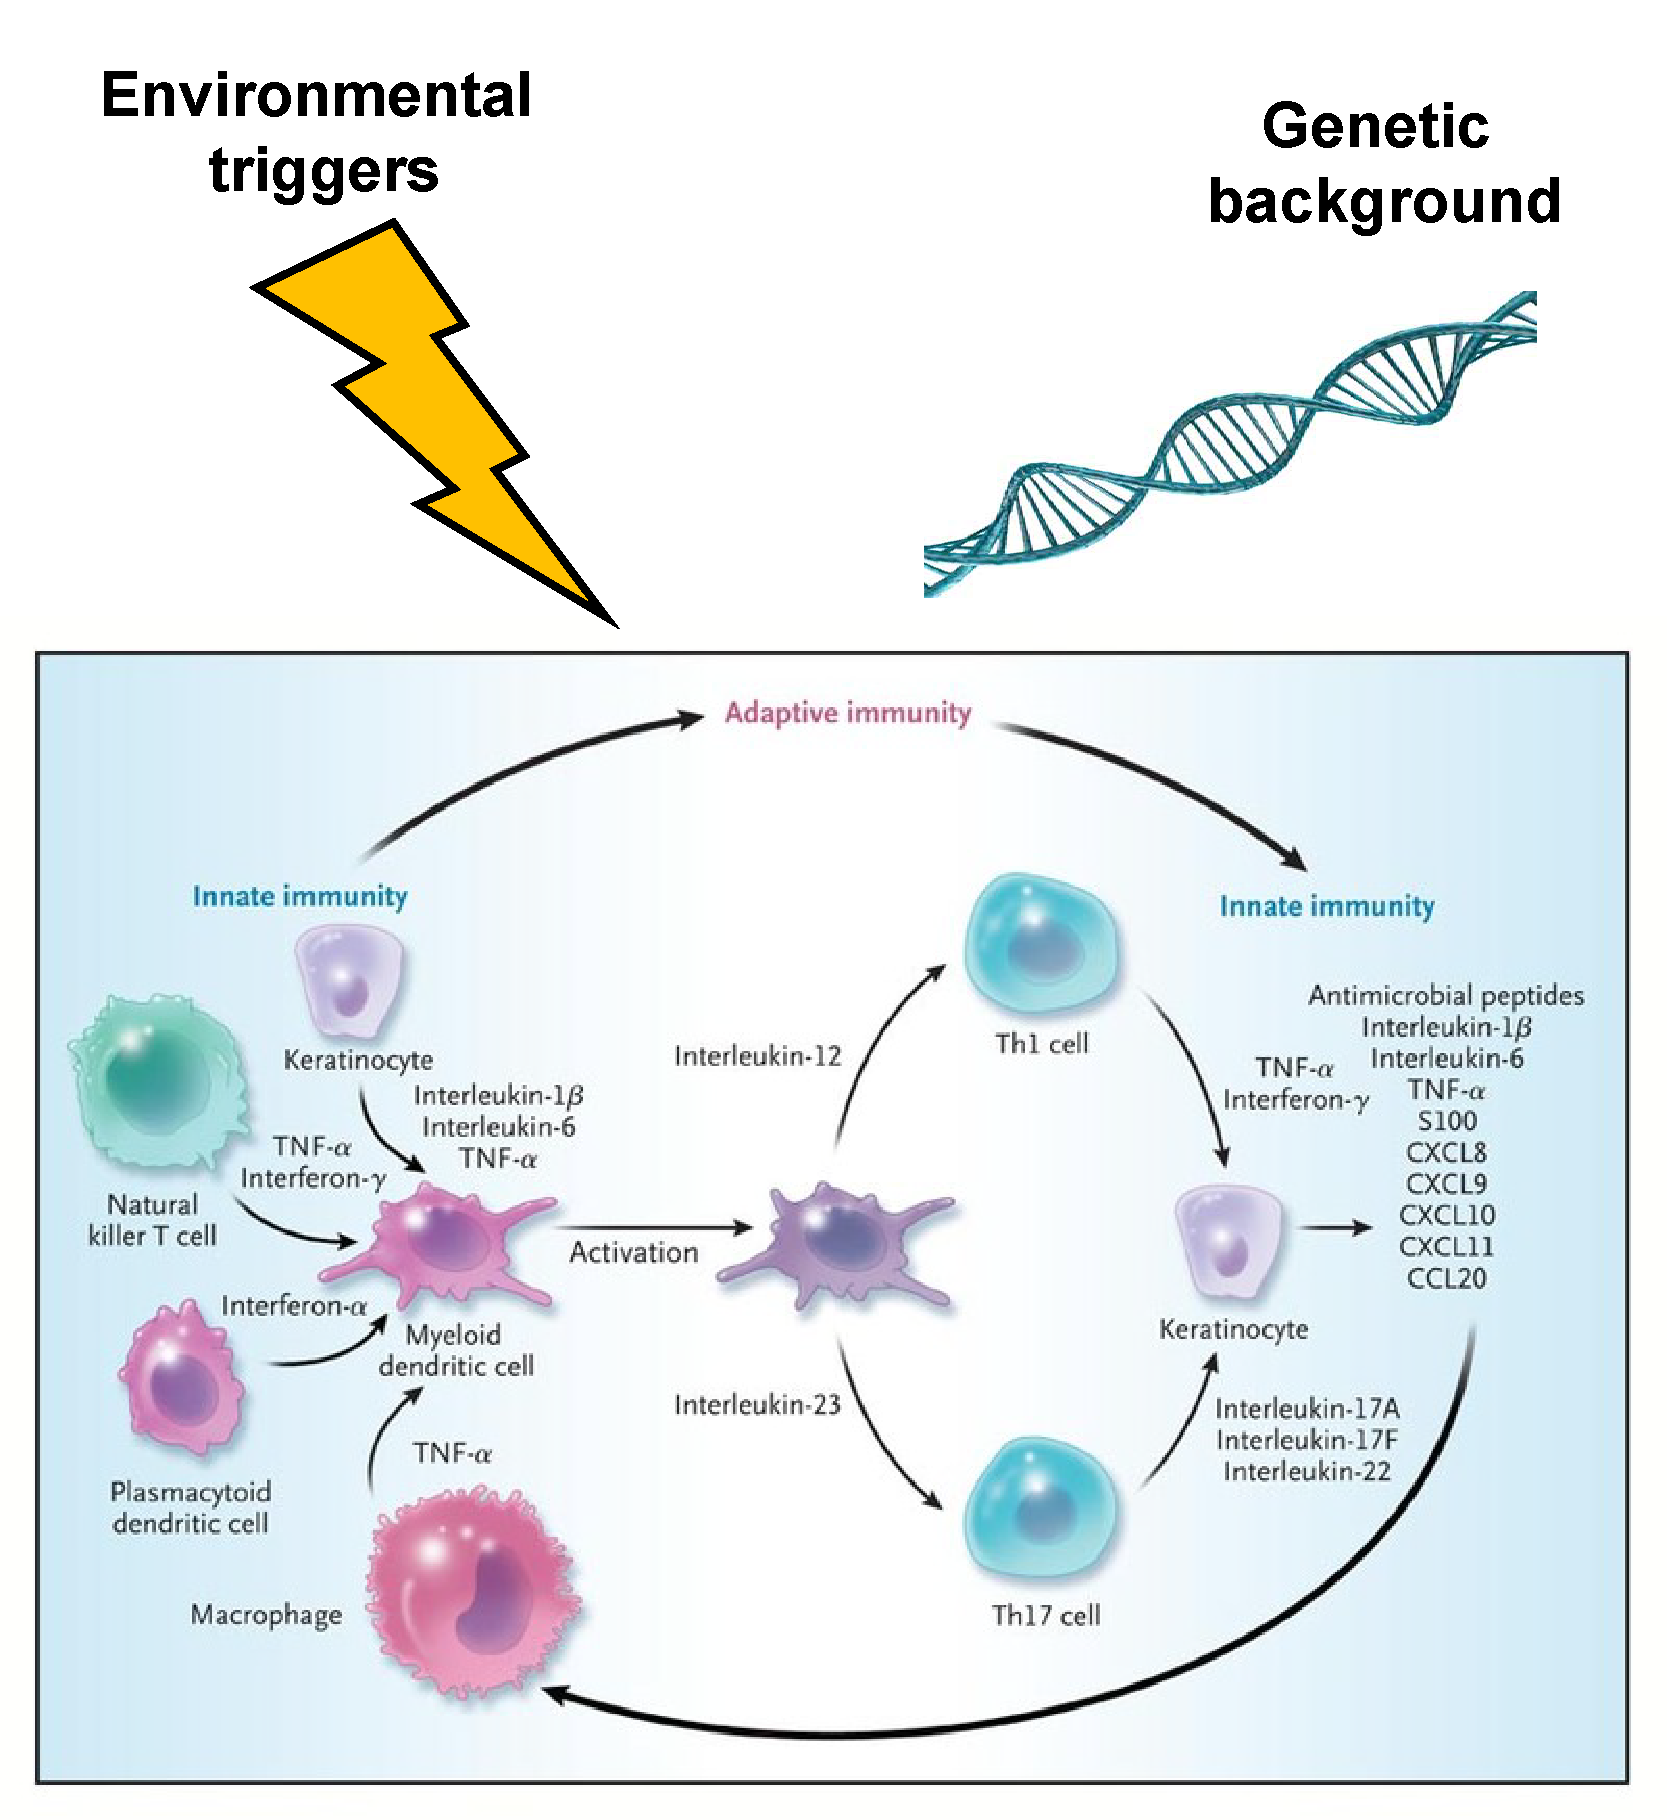
\includegraphics[width=0.8\textwidth]{./Introduction/pdfs/PSO_adaptive_innate_immune_system_crosstalk.pdf}
\caption[Crosstalk between innate and adaptive immunity in psoriasis]{\textbf{Figure adapted from \parencite{Nestle2009}}}
\label{fig:PSO_immune_system_diagram}
\end{figure}


Neutrophils are also though to be closely involved in disease initiation through their ability to form neutrophil extracellular traps (NET) that contain host DNA and LL-37 \parencite{Hu2016}. There is evidence of increased NET formation in peripheral blood and lesional skin of psoriasis patients and they seem to be contributing to pDC and CD4$^+$ T activation \parencite{Hu2016}. Neutrophils have also been identified in recent studies as one of the main sources of IL-17 production in the skin lesions \parencite{Lin2011} and they also release a wide range of proteases which some induce KC proliferation \parencite{Mahil2006}.


%HLA-Cw*06:02 can be recognised by the inhibitory receptor KIR2DL1 and the activatory receptor KIR2DS1.  Some studies have shown KIR2DS1 was present in 85\% of the patients but only in 51\% of the controls
%NK cells are important regulators of immune responses \parencite{Luszczek2004}. Their function extends beyond killing of infected or transformed cells. Interactions with dendritic cells, macrophages, and fetal trophoblast cells can regulate NK cell activity by influencing cytokine production, cytotoxicity and stimulation of T helper-1 responses. 
%
%


The involvement of monocytes and macrophages in psoriasis and PsA innate immunity has not been extensively explored. Resident macrophages in the healthy dermis undergo a 3-fold increase upon skin lesion and contribute to disease development through TNF$\alpha$ production \parencite{Perera2012, Mahil2016}. Similarly, mouse models for chronic psoriasiform skin inflammation have shown the role of macrophage migration into the affected skin and production of TNF-$\alpha$ in maintenance of the skin lesions \parencite{Stratis2006, Wang2006}. Initial studies showed greater phagocytic and bactericidal activity of peripheral blood mononuclear cells (PBMCs) isolated monocytes from psoriasis patients compared to those from healthy individuals \parencite{Bar-Eli1979}. Additionally, increased circulating intermediate monocytes (CD14$^+$ high CD16$^+$ high) and monocyte aggregation was also observed in psoriasis patients, resulting in enhanced platelet activation and angiogenesis \parencite {Golden2015}. In PsA synovial membranes, the levels of monocytes/macrophage metalloproteinases responsible for bone erosion through differentiation into osteoclasts  have been found to be similar to those found in rheumatoid arthritis (RA) joints \parencite{Hitchon2002}. 

Regarding the adaptive immunity, T lymphocytes have been considered the most relevant cell types in the initiation and maintenance of psoriasis and PsA. Report cases in humans have demonstrated that bone marrow transplantation can initiate or terminate psoriasis \parencite{Eedy1990, Gardembas1990}. Reduced numbers of circulating T cells but increased percentages of the memory populations CD4$^+$CD45RO$^+$ and CD8$^+$CD45RO$^+$ have been observed in moderate-to-severe and severe psoriasis patients when compared to milder phenotypes and healthy controls \parencite{Lecewicz-Toruń2001,Langewouters2008}. Different studies have reported controversial results regarding the total abundance and ratios of CD4$^+$ and CD8$^{+}$ in PBMC, likely due to the phenotype heterogeneity of the psoriasis cohorts between studies \parencite{Lecewicz-Toruń2001,Cameron2003,Langewouters2008}. In PsA, no differences in abundance of circulating T cells have been identified when compared to healthy individuals \parencite{Costello1999}.

In homeostasis, CD8$^+$ and CD4$^+$ lymphocytes are found in the epidermis and dermis, respectively \parencite{Clark2006}. An increase in activated memory CD4$^{+}$CD45RO$^{+}$and CD8$^{+}$CD45RO$^{+}$ cells can be detected by the third day from the lesion appearance \parencite{Clark2006,Perera2012}. \textit{In vivo} studies showed that development of psoriasis following engrafted human pre-lesional skin was only dependent on local T cell proliferation, highlighting the importance of circulating T cells recruitment during the priming event rather than at later stages of the disease \parencite{Wrone-Smith1996,Nickoloff1999,Perera2012}. The relative importance of CD4$^+$versus CD8$^+$ cells in psoriasis initiation has been explored in pre-lesional skin mouse xenografts where CD4$^+$ but not CD8$^+$ T cells were required in the transition from uninvolved to lesional skin \parencite{Nickoloff1999}. Interestingly, the injection of activated CD4$^+$ cells in mice was followed by an acute increase in activated resident CD8$^+$ T cells. Overall, these results supported the hypothesis of skin CD4$^+$ cells being drivers of resident T-cell activation and the population of resident activated CD8$^+$ the main effector of the immune response. In synovial tissues of PsA patients, CD4$^+$ are significantly more abundant than CD8$^+$ \parencite{Diani2015}. However, amongst the CD8$^+$ populations, the memory cells are prevalent in the patients’ synovial fluid (SF) with a significant enrichment compared their counterparts in PsA PB and RA SF\parencite{Costello1999}. The contribution of regulatory T (Treg) remains controversial in both, psoriasis and PsA \parencite{Perera2012}. 

Based on the cytokine profile, psoriasis and PsA have been classified as a type 1 Th/Tc disease, where activation of naive CD4$^+$ and CD8$^+$ cells is driven by IL-12 and IFN-$\gamma$ \parencite{Austin1999,Perera2012}. In addition, T-cell subsets including Th-17/Tc-17 and Th-22/Tc-22, producing high levels of IL-17 and IL-22, respectively, have been identified to be relevant for the perpetuation of the inflammatory response \parencite{Mahil2016}. The importance of Th-17 cells and IL-17 production has been evaluated in skin, joints and blood, with elevated mRNA and protein levels of IL-17 and also IL-23 reported in psoriasis and PsA patients compared to controls \parencite{Cai2012, Dolcino2015}. The relevance of IL-17 has been further highlighted by the presence of CD8$^+$ populations in patients’ SF that are predominantly IL-17 producers and whose abundance correlates with markers of inflammation and structural changes in the joint \parencite{Menon2014}. This finding is in line with observations in skin and suggests a prominent role for CD8$^+$ IL-17-producing cells in the different stages of both pathologies. Studies directed to understand the importance of IL-17 have led to the discovery of other immune cells producing this pivotal cytokine, including innate immune lymphoid (ILC) cells and $\gamma$$\delta$ T cells, opening new research avenues in the context of psoriasis and PsA pathophysiology and treatment \parencite{Meglio2014,Leijten2015}. IL-17-producing cells have also been hypothesised to be at the link between skin and joint lesions. Although the precise mechanisms for transition between psoriasis and PsA is still poorly understood, the study of psoriasis and RA in mouse models revealed that skin lesions facilitate arthritis and joint inflammation \parencite{}. %In fact, the presence of IL-17-producing cells in the inflamed skin nearby the enthesis of joints under physical stress is likely to be a trigger for the development of PsA.



\subsection{Therapeutic intervention}
Ppsoriasis and PsA are currently incurable diseases, with the different treatments available solely focused on alleviating the symptoms. For instance, topical therapies are advocated in cases of mild-to-moderate psoriasis, represented by extended emollients and short-term corticosteroids, due to associated side-effects \parencite{Menter2009}. Other treatments may be used in combination with corticosteroids, such as ultraviolet (UV) light therapy and vitamin D analogues, directed to inhibit T-cell and KC proliferation and stimulate KC differentiation \parencite{Rizova2001}. In the case of PsA patients presenting with swelling of two or fewer joints, intra-articular injection of glucocorticosteroids together with joint aspiration is used as a short-term solution to reduce pain and inflammation \parencite{Coates2016}. However, treatment of most forms of PsA and moderate-to-severe psoriasis require the use of systemic therapies. Patients presenting with mild cases of PsA commonly receive nonsteroidal anti-inflammatory drugs (NSAID) to control the inflammatory symptoms \parencite{Coates2016}. More severe forms of PsA require the use of disease-modifying antirheumatic drugs (DMARDs) including the antagonist of folic acid methotrexate (MTX) and the phosphodiesterase 4 inhibitor Apremilast, which act as immunosuppressors of activated T cells and cytokine production, respectively \parencite{Schmitt2014, Gossec2016, Keating2017,Polachek2017}.

Remarkably, biologic systemic agents represent the most specific treatment option for severe psoriasis and PsA. This category encompasses an array of cell-based molecular species that modulate the immune response in a physiological manner \parencite{Perera2012}. Specifically, the relevance of TNF-alpha in psoriasis and PsA has led to the extensive therapeutic use of TNF-alpha inhibitors (TNFi) during the past five decades, making them the ‘drugs of choice’ amongst all the biologic agents targeting cytokine pathways. Three TNFi have been approved for the treatment of psoriasis: etanercept, infliximab and adalimumab \parencite{Ahil2016}. In addition to those, certolizumab pegol and golimumab are often used in the management of PsA and other rheumatoid diseases \parencite{Coates2016b}. Despite TNF-$\alpha$ blockade being one of the most effective treatments, side effects such as increased risk of infection or reactivation of latent infections have been identified \parencite{Nickoloff2004}. Moreover, between 20 to 50\% of patients fail to respond to the first TNFi administrated, requiring switching to an alternative TNFi \parencite{Abramson2016}. New biologic therapies have been developed to target other key cytokines, such as IL-12, IL-23 (ustekinumab) or IL-17 (secukinumab and ixekizumab), which represent a substantial advance in treating patients failing to respond to TNFi \parencite{Mahil2016, Coates2016b}.

% Bispecific antibodies

 

\section{Genetics of psoriasis and psoriatic arthritis}

As complex diseases, the risk of developing psoriasis and PsA is not only influenced by environmental conditions but also by the genetic background of each individual. Determining the magnitude of the contribution of genetic factors in the development of these diseases and identifying the exact genes or genomic regions involved in the predisposition to psoriasis and PsA remains challenging.  Several studies have shown an increase in psoriasis and PsA prevalence over the last 30 years in different countries \parencite{Organization2016}. This importantly reflects changes in life style habits and it highlights the need to better understand the genetic factors that predispose to disease upon interaction with environmental stresses.


\subsection{Heritability}

The contribution of genetics in the development of psoriasis has been demonstrated in several twins studies. The concordance of psoriasis is greater in monozygotic (33-55\%) compared to dizyogtic twins (13-21\%), giving a heritability estimate of 80\% in this condition \parencite{Faber1974, Duffy1993, Pendersen2008}. Conversely, similar concordance across mono- and di- zygotic twins has been reported in the case of PsA, probably due to lack of statistical power and appropriate diagnosis \parencite{Pendersen2008}. In the general population, approximately 40\% of patients with psoriasis or PsA have family history in first degree relatives \parencite{Gladman1986}. Interestingly, the recurrence rate in first-degree relatives has been shown to be greater in PsA (40\%) compared to psoriasis (8\%) in a study in the Icelandic population \parencite{Chandran2009}. This suggests differences in the heritability between the two phenotypes and a stronger genetic contribution in PsA.


\subsection{Non-GWAS and linkage studies}

The study of psoriasis and PsA genetic architecture started with linkage analyses in family pedigrees presenting an autosomal dominant condition. This approach yielded nine psoriasis susceptibility loci (PSORS1-9) with PSORS1 showing the strongest genetic association \parencite{Capon2017, International2003}. PSORS1 locus lies within the MHC I region in chromosome 6p21, previously associated with psoriasis susceptibility in serological studies \parencite{Rusell1972, Tiilikainen1980}. Importantly, Mendelian forms of disease with rare highly penetrant mutations have also been identified in family studies for two genes within PSORS2 (17q25): zinc finger protein 750 (\textit{ZNF750}) and caspase domain family member 14 (\textit{CARD14}) \parencite{Tomfohrde1994,Jordan2012}. Rare gain of function and \textit{de novo} mutations together with common variants in \textit{CARD14} have been identified in psoriasis and PsA patients, suggesting an important role of genetic variation in this gene in Mendelian and multi-factorial forms of disease \parencite {Jordan2012, Tsoi2012}. %In PsA, a region close to the psoriasis PSORS8 was also identified \parencite{Karason2003}.
 Additionally, gene based studies in psoriasis and PsA disclosed the importance of genetic variability in the activating killer immunoglobulin receptors 2DS1 (\textit{KIR2DS1}) gene, also reported for AS and RA, which interestingly is mainly triggered by interaction with HLA-Cw*06:02 \parencite{Łuszczek2004, Williams2005,Carter2007, Yen2001}.  Nevertheless, the inability of independent studies to reproduce these results for regions other than PSOR1, 2 and 4, highlights the limitations of linkage studies to understand the genetics of complex diseases \parencite{Capon2017}. 

%Similarly, specific association with PsA but not psoriasis was found for microsatellites and promoter polymorphisms in TNF-$\alpha$ \parencite{H\"{o}hler2002}. 


\subsection{Genome-wide association studies}

Recent dramatic advances in sequencing and genotyping technologies have allowed the implementation of association studies at a genome-wide scale. Genome-wide association studies (GWAS) have benefitted from the understanding of common single base-pair changes known as single nucleotide polymorphisms (SNPs) in different populations through whole genome sequencing (WGS) projects such as HapMap \parencite{The international HapMaP Consortium} and the 1000 Genomes Project \parencite{The 1000 Genomes}. GWAS generally focus on identifying disease-associated common SNPs (with minor allele frequency (MAF) ${>}$5\% ) showing differences in allele frequency between patients and controls \parencite{Ku2010}. GWAS are thus based on the hypothesis that complex diseases are caused by the interaction of multiple common variants, and are designed to have greater power than the previous linkage studies to identify multiple loci with low penetrance and moderate to small effects \parencite{Schork2009, Cui2010}. 

%Due  to the organisation of the genome into segments of strong linkage disequilibrium (LD) where genetic variants are strongly correlated with each other, the genotyped SNPs in GWAS are solely used a proxy for the disease causative variant. Therefore, disease causal variants can be non-genotyped SNPs or other type of genetic variability such as copy number variants (CNVs), also highly frequent in the genome but less widely studied by GWAS \parencite{Hirschhorn2005, Ku2010}. 
The genotyped SNPs in GWAS are solely used a proxy for the disease causative variant, for instance non-genotyped SNPs or other type of genetic variability such as copy number variants (CNVs) \parencite{Hirschhorn2005, Ku2010}.
Since 2007, when the first psoriasis and PsA GWAS were published, a total of sixty-three genetic associations have been identified at a genome-wide significance (pval$>$5x10$^-8$) which explain 28\% of the psoriasis and PsA heritability (Table \ref{tab:GWAS_studies}) \parencite{Tsoi2017}. The majority of studies have been performed in Caucasian European or North American cohorts but increasing numbers of GWAS in large Chinese cohorts are also being published \parencite{Zhang2009, Sun2010, Yin2015}. The early GWAS performed in discrete size cohorts with moderate power confirmed association with loci overlapping the PSOR1 and PSOR2 genomic regions identified in the linkage studies \parencite{Cargill2007,Strange2010}. Specifically, HLA-C has been consistently identified as the most significant locus with the greatest effect size. Additional MHC-I and MHC-II associations with disease risk have been identified for HLA-A, HLA-B and HLA-DQA1 through step-wise conditional analysis\parencite{Okada2014}. 
The information extracted from GWAS studies was significantly enhanced with the use of the Immunochip genotyping platform, which covers 186 immune relevant loci identified in previous GWAS studies across different inflammatory diseases at a greater genotyping density \parencite{Tsoi2012}. The psoriasis Immunochip study uncovered fifteen new associations, including the PSOR4 \textit{CARD14} and also included meta-analysis with the largest available psoriasis cohorts at the time\parencite{Tsoi2012}. This meta-analysis has been further expanded yielding sixteen additional associations in the latest study and reinforcing the importance of NF$\kappa$B and cytotoxicity pathways in disease pathophysiology \parencite{Tsoi2015,Tsoi2017}. Meta-analysis of GWAS across Caucasian and Chinese populations has demonstrated the value of this trans-ethnic approach to identify new associations and understand the differences in the genetic associations contributing to disease risk in different populations \parencite{Yin2015}. 
%Four new non-coding loci in the vicinity of \textit{LOC144817}, \textit{COG6}, \textit{RUNX1} and \textit{TP63} were associated with psoriasis and PsA in both populations. Interestingly, genetic heterogeneity between Caucasian and Chinese cohorts was also observed for ten of the GWAS reported loci, for example \textit{ELMO1} and \textit{TYK2}.
The importance of conducting independent GWAS studies for psoriasis and PsA has been shown not only by the discrepancy in first degree relatives heritability but also by differences in HLA-C and HLA-B alleles frequencies within each phenotype population \parencite{Winchester2012, Okada2014}. In fact, cohort stratification confirmed specific GWAS association with PsA for previously identified psoriasis loci such as \textit{TRAF3IP}, \textit{IFNLR1}, \textit{IFIH1} and \textit{NFKBIA} as well as PsA-specific independent signals for \textit{IL23R} and \textit{TNFAIP3} \parencite{Ellinghaus2010, Stuart2015}.  Interestingly, the association for \textit{LCE3C/B}, identified in combined phenotypic studies, showed greater strength in those patients presenting psoriasis for over ten years without developing joint affection \parencite{Stuart2015}. Lately, PsA GWAS using the Immunochip platform revealed a PsA-specific association in chromosome 5q31 and an independent secondary signal in the \textit{IL23R} region \parencite{Bowes2015}. 




%
\begin{landscape}
\begin{center}
\begin{longtable}[ht]{p{.25\textheight} p{.25\textheight} p{.20\textheight} p{.20\textheight} p{.50\textheight}}
%{p{.15\textheight} p{.15\textheight} p{.25\textheight} p{.25\textheight} p{.15\textheight} p{.15\textheight} p{.15\textheight}}
\caption[Main GWAS studies in psoriasis and PsA]{\textbf{Main GWAS studies in psoriasis and PsA.} Summary table describing the most relevant psoriasis and PsA GWAS studies. Information regarding sample size, patients phenotypes and the main reported associations in each study is included. The Ellinghaus \textit{et al.}, 2010 and the Stuart \textit{et al.}, 2015 studies included stratified association analysis of psoriasis and PsA independently. WA=white American; Eur=European; $^\star$ Meta-analysis performed.}
\label{tab:GWAS_summary} \\
\toprule
\textbf{Study} & \textbf{Etnicity} & \textbf{Sample size}      & \textbf{Phenotype} & \textbf{Main associations} \\
               &                   & \textbf{(Cases/Controls)} &                    &  \textbf{(putative genes)}                  \\
\midrule
\midrule
\parencite{Cargill2007} &	WA &	1,446/1,432 &	Psoriasis, PsA &	HLA-C (PSOR1) and \textit{IL12B} \\
\parencite{Nair2009} &	Eur	& 1,409/1,436 &	Psoriasis, PsA &	\textit{IL23A}, \textit{IL23R}, \textit{IL12B}, \textit{TNIP1}, \textit{TNFIP3}, \textit{IL4} and \textit{IL13} \\
\parencite{Stuart2010} &	WA, Eur &	1,831/2,546	& Psoriasis, PsA &	\textit{NOS2}, \textit{FBXL19},\textit{PSMA6-NFKBIA} \\

\parencite{Ellinghaus2010} &	German	& 472/1,146	& Psoriasis	& \textit{TRAF3IP2} \\

\parencite{Strange2010} &	Eur & 2,622/5,667 & Psoriasis, PsA & \textit{LCE3D} (PSOR2), \textit{IL28RA}, \textit{REL}, \textit{IFIH1}, \textit{ERAP1}, \textit{TYK2} and \textit{HLA-C/ERAP1} epistasia \\

\parencite{Zhang2008} & Chinese	& 1,139/1,132	& Psoriasis (type I)  & \textit{LCE} gene family and \textit{IL12B} \\

\parencite{Sun2010} & Chinese	& 8,312/12,919	& Psoriasis, PsA &	\textit{ERAP1}, \textit{PTTG1}, \textit{CSMD1}, \textit{GJB2}, \textit{SERPINB8} , \textit{ZNF816A} \\

\parencite{Tsoi2012}$^\star$ & WA, Eur & 10,588/22,806 & Psoriasis, PsA & \textit{CARD14} (PSOR4), \textit{RUNX3}, \textit{B3GNT2}, \textit{ELMO1}, \textit{STAT3} \\

\parencite{Tsoi2015}$^\star$	& WA, Eur	& 15,000/27,000	& Psoriasis, PsA	& 1q31.1, 5p13.1, \textit{PLCL2}, \textit{NFKBIZ}, \textit{CAMK2G} \\

\parencite{Bowes2015} &	British, Irish, Australians	& 1,962/8,923	& PsA	& 5q31 PsA-specific \\

\parencite{Stuart2015} &	WA and Eur	& 1,430/1,417	& Psoriasis, PsA	& PsA-specific secondary signals (main text), 1p36.23 psoriasis-specific, stronger psoriasis \textit{LCE} association\\

\parencite{Yin2015} &	WA, Eur, Asian	&  15,369/19,517 & Psoriasis, PsA	& \textit{LOC144817}, \textit{COG6}, \textit{RUNX1} and \textit{TP63}; signals with ethnic heterogeneity \\

\parencite{Tsoi2017}$^\star$ &	WA, Eur	& 19,032/39,498	& Psoriasis, PsA	& \textit{CHUK}, \textit{IKBKE}, \textit{FASLG}, \textit{KLRK1}, \textit{PTEN} \\																		
\bottomrule
\medskip
\end{longtable}
\end{center}
\end{landscape}


Overall, GWAS studies have demonstrated shared genetic susceptibility between psoriasis and PsA, but have also highlighted intrinsic specificity that may support a difference in the genetic architecture of both diseases. It is important to take into account that these results are affected by imprecise phenotyping of cases, which is one of the many challenges in the systematic comparison between the two diseases.

\subsection{Relevance of non-coding variants in disease susceptibility}

Approximately 88\% of all GWAS associations map within non-coding regions, withonly the remaining 12\% comprising non-synonymous coding mutations impacting the protein function \parencite{Welter2013}. Psoriasis exome association studies in Chinese and Caucasian populations have increased the number of coding variants with putative effects on the protein structure \parencite{Tang2014, Zuo2015, Dand2017}. These studies have confirmed some  previously identified missense associations in \textit{CARD14} and \textit{ERAP1}, revealed new common coding variants at these previously associated loci and identified rare protective missense changes, for example in the \textit{TYK2} gene\parencite{Tang2014,Dand2017}. Nevertheless, results from extensive exome studies suggest that non-synonymous SNPs have a limited contribution to the overall genetic risk of psoriasis compared to non-coding variants \parencite{Tang2014}.

The association of non-coding variants with disease can be explained by their ability to regulate gene expression in a cell and context specific manner \parencite{Fairfax2012}. These variants can be located in different regulatory elements, including enhancer, silencers, promoters and the 5' and 3' untranslated region (UTR) of genes \parencite{Ward2012}. Non-coding GWAS variants can alter the expression of target genes through different mechanisms including changes in chromatin accessibility, histone modifications, protein binding such as transcription factors (TFs), DNA methylation and binding of non-coding  RNA molecules\parencite{Knight2014} (\ref{subsec:Epigenetics}).

Identification of the target gene regulated by non-coding variants represents a challenge in the field of functional genetics. This limitation can be partially addressed by conducting expression quantitative trait loci (eQTL) analysis, which identifies genome-wide statistical associations between gene transcript levels and SNPs in \textit{cis} ($<$1Mb) or \textit{trans} to the gene. For instance, in T2D an such approach revealed a \textit{cis}-eQTL involving the TF \textit{KLF4} and a haplotype of non-coding GWAS SNPs located 14kb up-stream \parencite{Small2011}. Moreover, this haplotype also showed association with genes in \textit{trans}, highlighting downstream targets regulated by KLF4. Nonetheless, eQTL mapping alone only provides statistical suggestion of transcriptomic regulation, and additional functional assays, such as chromatin conformation, are required to demonstrate causality \parencite{Edwards2013}.  
 


\subsection{The role of GWAS studies in highlighting immune-relevant cell types and pathways}

GWAS represent a biologically unbiased approach to shed some light on pathophysiological relevant cell types and molecular pathways associated with disease. In the field of common immune-mediated diseases, GWAS have underlined some of the most important cell types for which genetic variation is functionally relevant. Better understanding of immune-related diseases has likewise led to identification of shared susceptibility loci and the use of therapeutic interventions across diseases, such as anti- IL-23 and anti- IL-17 antibodies to treat psoriasis, PsA, AS and IBD \parencite{Visscher2017}.

Systematic comparison of the genetic architecture across different conditions has revealed psoriasis and PsA risk loci to be shared, in the same or opposite directions, with AS, CD, MS, RA and T1D \parencite{ImmunoBase}. Interestingly, cross-disease association studies performed for AS, UC, primary sclerosing cholangilitis (PSC), CD and psoriasis has revealed significant overlap  of the multi-trait associated loci in regulatory elements in bone marrow, NK and T cells as well as immune response pathways \parencite{Ellinghaus2016}. %This study also identified genetic pleiotropy of psoriasis with AS and CD, illustrating how the same alleles can predispose individuals for different diseases, and demonstrating the contribution of GWAS to the biological understanding of disease.

In the case of psoriasis and PsA, the majority of GWAS risk loci have been linked to genes that belong to a limited number of pathways and show enrichment for regulatory elements in several cell types \parencite{Capon2017}. 


\subsubsection*{Antigen presentation}
In psoriasis \textit{HLA-Cw*0602} represents the strongest GWAS association,  shared with other diseases such as Hepatitis C, PSO and Grave´s disease \parencite{Blais2011}. No differences at the transcript level have been identified for HLA-Cw*0602 when comparing psoriasis patients versus controls, suggesting alterations in antigen presentation as the mechanism explaining disease association \parencite{Hundhausen2012}. The relevance of antigen presentation in psoriasis and PsA has been reinforced by the GWAS association of the endoplasmic reticulum aminopeptidase 1 \textit{ERAP1} gene, involved in the trimming of peptide antigens. Moreover, GWAS studies identified that \textit{ERAP1} was associated with psoriasis and PsA only in individuals carrying one copy of the rs10484554 \textit{HLA-C} risk allele \parencite{Strange2010}. Similarly, the same study identified a dependent association between \textit{HLA-Cw*0602} and SNPs in the vicinity of the zeta chain of T cell receptor associated protein kinase 70 (\textit{ZAP70}) gene \parencite{Picard2009}.% involved in the regulation of CD8$^+$ cells auto-reactivity 
These epistatic phenomena, whereby association of one gene is dependent on the presence of another, have also been reported between \textit{HLA-B*27} and \textit{ERAP1} in AS \parencite{Evans2011, Cortes2015b}. Interestingly, the AS \textit{ERAP1} GWAS association increases \textit{ERAP1} expression and also alters splicing, resulting in an ERAP1 protein isoform with increased activity \parencite{Constatino2015, Hanson2018}.%which shares signal and direction with psoriasis


\subsubsection*{Skin barrier}

GWAS have highlighted KC specific genes such the previously mentioned \textit{LCE} gene cluster and genes with a key role in skin biology such as \textit{CARD-14}. Further studies in the \textit{PSORS4} region have revealed that association with disease is driven by a deletion in two of the genes within this family, \textit{LCE3B} and \textit{LCE3C} (\textit{LCE3C$\_ $LCE3B$\_ $del})\parencite{Cid2009}. %Expression of \textit{LCE3B} and \textit{LCE3C} is induced upon barrier disruption, where these proteins participate in the formation of the cornified envelope at the most external layer of the epidermis and are likely involved in KC terminal differentiation \parencite{Bergboer2011}. 
The lack of \textit{LCE3B} and \textit{LCE3C} expression in psoriasis patients could lead to impaired repair following skin disruption, potentially facilitating microorganism infection and triggering a dysregulated immune response \parencite{Bergboer2011}. In fact, the use of UVB radiation has been shown to upregulate \textit{LCE3E} expression 48 hours after treatment, contributing to amelioration of the skin lesions\parencite{Jackson2005}. % Interestingly, epistasia between this deletion and \textit{HLA-Cw*0602} has also been identified in Dutch and American populations amongst others \parencite{Cid2009, Riveira-Munoz2011}. 
Similarly to the \textit{LCE} gene cluster, \textit{CARD14} is primarily expressed in epithelial tissues mediating the recruitment and activation of the NF-$\kappa$B pathway in this tissue \parencite{Blonska2011}. Common and rare pathogenic mutations of \textit{CARD14} in KC cell lines lead to increased activation of NF-kB as well as overexpression of psoriasis-associated genes including \tetxit{IL6}, \textit{TNFA} and \textit{TNFAIP2}, among others \parencite{Jordan2012b}.
%https://www.sciencedirect.com/science/article/pii/S0002929712001577?via%3Dihub



\subsubsection*{NF-$\kappa$B and TNF pathways}

The NF-$\kappa$B pathway is involved in the regulation of the innate and adaptive immune response. In fact, dysregulation of the feedback loop between TNF-$\alpha$ and NF-$\kappa$B contributes to the development of many chronic inflammatory diseases, being the neutralisation of TNF-$\alpha$ widely used for treatment of immune-mediated diseases, as previously detailed \parencite{Liu2017}. In psoriasis, for example, elevated levels of NF-$\kappa$B are present in lesional compared to uninvolved and normal skin \parencite{Lizzul2005}. 

Several psoriasis and PsA GWAS loci have been mapped to gene members of the NF-$\kappa$B and TNF signalling pathways including \textit{TNIP1}, \textit{TNFAIP3}, \textit{NFKBIA}, \textit{REL}, \textit{TRAF3IP2}\parencite{Nair2008, Ellinghaus2010, H\"{u}ffmeier2010, Wang2008, Idel2003, Bowes2012}. 
%\textit{NF-$\kappa$B} is a dimeric TF that translocates into the nuclei upon cytokine stimuli, including TNF-$\alpha$ itself. 
For example, a haplotype including missense mutations and intronic variants in \textit{TRAF3IP2} has been reported to drive psoriasis and PsA association by reducing its affinity for TRAF interacting proteins and concomitantly altering NF-$\kappa$B activation and the IL-17/IL-23axis\parencite{H\"{u}ffmeier2010, Ellinghaus2010}. SNP variants in the \textit{TRAF3IP2} locus have also been identified in CD and UC, reinforcing the relationship between these two pathways and chronic inflammation \parencite{ImmunoBase}. In addition, exome-sequencing studies have identified variants with predicted influence on protein structure and function at \textit{TNFSF15}, a TNF ligand family protein induced by TNF-$\alpha$, with a primary role in regulating NF-$\kappa$B and MAP kinases activation in endothelial cells \parencite{Dand2017, Wang2014}.

The psoriasis and PsA GWAS associations with other members of these pathways, such as the NF-$\kappa$B inhibitor \textit{NFKBIA} and the NF-$\kappa$B subunit \textit{REL}, are solely supported by proximity to nearby intergenic SNPs, with no direct experimental evidence for a role of these genetic variants in regulating the expression of either gene \parencite{GWAS studies}. Moreover, the latest psoriasis and PsA meta-analysis study revealed three additional associations with genes belonging to the NF-$\kappa$B pathway (\textit{CHUK}, \textit{IKBKE} and \textit{FASLG}), further implicating NF-$\kappa$B activation in psoriasis and PsA development \parencite{Tsoi2017}.
%The hypothesised psoriasis and PsA GWAS association with the NF-$\kappa$B inhibitor \textit{NFKBIA} and the NF-$\kappa$B subunit \textit{REL} are solely supported by proximity to nearby intergenic SNPs, with no direct experimental evidence for a role of these genetic variants in regulating the expression of either gene \parencite{GWAS studies}. \textit{REL} has been associated with other inflammatory diseases, including CD and RA \parencite{ImmunoBase} although interestingly, the RA risk allele has a protective effect in PsA \parencite{Bowes2012}. 

%The relevance of genes downstream of TNF-$\alpha$ signalling is highlighted by GWAS associations with \textit{TNIP1} and \textit{TNFAIP3}, which participate in the regulation of NF-$\kappa$B activation. For example, knock-in of a region including \textit{Tnfaip3} induces psoriasis in mice and increases the risk of athresoclerosis, one of the most prevalent co-morbidities in psoriasis and PsA \parencite{Wang2008, Idel2003}. Nevertheless, reported immune related pathologies due to constitutive deficiency in NF-$\kappa$B highlights the lack of drugability of this target \parencite{Orange2005,Puel2004}



\subsubsection*{Type I IFN and innate host defense}
Psoriasis and PsA GWAS associations have highlighted genes involved in innate immunity including the host response to viruses and bacteria, importantly represented by members of the type I IFN signalling pathway. Mapping of several GWAS loci to genes from the type I IFN signalling pathway together with clinical and experimental data has reinforced the role of pathogen response in psoriasis and PsA \parencite{Nestle2005}. GWAS associations involved in this IFN response include \textit{IL28RA}, \textit{IFIH1}, \textit{TYK2}, \textit{RNF114}, \textit{ELMO1} and \textit{DDX58}, some of which have been previously reported as susceptibility loci for other immune-mediated diseases (\ref{tab:GWAS_summary}). For instance, GWAS-lead SNPs causing missense mutations in \textit{TYK2} have been identified in CD, IBD, T1D, RA and MS, in addition to psoriasis and PsA \parencite{ImmunoBase}. % \textit{TYK2} is a Janus kinases (JAK) protein member that initiates the IFN type I downstream response \parencite{Calamonici1994}. 
Exome-sequencing and GWAS studies have identified two independent protective missense mutations predicted to impair the catalytic activity of the Janus kinases (JAK) protein member TYK2, and thus the initiation of the IFN-I downstream inflammatory cascade in psoriasis and PsA \parencite{Strange2010, Tsoi2012, Dand2017}. A JAK inhibitor approved solely for use in RA treatment, is currently undergoing clinical trials in other immune-related diseases alongside the development of more specific JAK inhibitors \parencite{Baker2017}. Moreover, drugs targeting upstream type I IFN pathway members, such as inhibitors of the pathogen-sensing receptors \textit{TLR7} and \parencite{TLR9}, are being conducted in SLE and may be extended to other immune-mediated diseases \parencite{Baker2017}. 
%For example, monoclonal Ab against IFN-$\alpha$ subtypes have failed to suppress the IFN gene signature in psoriasis patients and new approaches towards blocking the IFN-$\alpha$ receptor have shown greater efficacy in SLE \parencite{Furie2017}. Psoriasis and PsA GWAS associations with upstream elements of the IFN I pathway such as intronic variants in \textit{ELMO1} gene may distort the activation of the pathogen-sensing receptors \textit{TLR7} and \parencite{TLR9} and hence IFN-$\alpha$ production in pDC \parencite{Tsoi2012}.Clinical trials testing inhibitors of these TLR receptors are being conducted in SLE \parencite{Baker2017}.
%IFNGR for type II IFN inhibition could be added

\subsubsection*{IL-17/IL-23 axis}
Together with the TNF pathway, the IL-17/IL23 axis is the most common target of biological therapeutics. In fact, some studies have reported greater efficacy of individual IL-17A or IL-23 blockade compared to TNF inhibition in the treatment of psoriasis and PsA \parencite{Griffiths2015,Blauvelt2017}. 
The cytokine IL-23, involved in a wide range of pro-inflammatory processed as previously explained, is formed of two subunits: IL-23A/p19 and IL12-B/p40, the latter also being a component of IL-12 protein. Transcriptional studies have shown increased levels of p40 and p19 in psoriasis lesional skin and a role for both subunits in abnormal KC differentiation \parencite{Lee2004,Zhu2011}. Psoriasis and PsA GWAS associations with the \textit{IL23R} have been reported in several studies, including a protective two SNP haplotype shared with CD in a German and American Caucasian cohort study \parencite{Nair2008, Strange2010, Tsoi2012}. GWAS associations have also been established by proximity of non-coding lead SNPs to \textit{IL23A} and \textit{IL12} genes, but direct functional evidence in regulation of their expression has not yet been established \parencite{Cargill2007,Strange2010,Tsoi2012}.
%Under inflammatory conditions, the arginine to glutamine (Arg381Gln) exchange in the IL23R showed a protective effect in CD \parencite{Duerr2006}. Conversely, this haplotype is not associated with psoriasis risk in Chinese population where a different non-synonymous potentially damaging variant has been reported as the putative mechanisms \parencite{Tang2014}.
Interestingly, an \textit{IL23} signal secondary to that reported by Tsoi \textit{et al.,} 2012 has been specifically associated with PsA, and independence from AS secondary signals for the same locus has also been demonstrated \textit{Tsoi2012,Bowes2015}. 
Regarding the genetics of the Th-17 pathway, its relevance is partly explained through the cross-talk with the IL-23 response, which mediates Th-17 cell differentiation and activation. Additionally, GWAS associations with intronic variants at TFs regulating the Th-17 polarisation, such as \textit{IRF4} and \textit{STAT3}, have also been identified for psoriasis and PsA \parencite{ Tsoi2012,Huber2008,Harris2007}. 
%These GWAS associations are also reported for other immune-mediated disease including CD and MS \parencite{, Immunobase}. Moreover, previously mentioned GWAS associations in the NF-$\kapa$B and TNF pathways such as \textit{TRAF3IP2}, \textit{NFKBIZ} and \textit{TYK2} are also shared with the IL-23/IL-17 axis, stressing not only the relevance of this pathway but also the importance of pathway cross-talk. 
% Interestingly, the inhibition of IL-17A using secukinumab is effective in the treatment of psoriasis, PsA and AS, whereas it worsens CD for which the treatment using antibodies against IL-12/23p40, as the previously mentioned ustekinumab, have a much prolonged benefit compared to the other diseases \parencite{Patel2012,Hueber2012,Blauvelt2017b} .Overall, this stresses the importance of the Th17/IL-23 axis in inflammation and demonstrates that blocking the pathway at different levels translates into different effects within and across inflammatory diseases.  

\subsubsection{Genome-wide pathway enrichment analysis and intergenic regions}

New approaches using genetic association data have allowed to perform genome-wide pathway analysis to disclose relevant biological processes in disease. %This analysis represents a more powerful and biological meaningful way than GWAS to study the association of functionally related genes with disease risk. 
In psoriasis, genome-wide pathway analysis has revealed association of novel processes, such as retinol metabolism, transport of inorganic ions and aminoacids and post-translational protein modifications (PTMs) not previously related with the disease aetiology \parencite{Aterido2015}. 

As previously mentioned, the majority of the non-coding GWAS associations are located at intergenic regions and often lack of functional characterisation. Therefore these variants tend to be associated to the nearest gene within few Kb away and which function is known and in line with current understanding of the pathophysiology. Nevertheless, some of these intergenic non-coding SNPs are located at regions depleted of genes for 300Kb or more. Some examples in psoriasis and PsA include chr1p36.23, chr2p15 and chr9q31.2. One of the most interesting regions is chr2p15, which lead SNP and direction of association is shared with AS \parencite{Immunobase}. Within this locus, genes with a role in the immune response involve \textit{B3GNT2} and \textit{CMMD1}, which are located at approximately 130Kb and 200Kb away from the GWAS lead SNP, respectively  \parencite{Maine2007, Tsoi2012}. Interestingly, the \textit{B3GNT2} gene was identified by the aforementioned genome-wide pathway analysis to contribute to the significant enrichment of the post-translational protein modifications pathway.
%Among the other intergenic associations chr1p36.23 is shared with UC and chr6q25.3 has also been reported in MS, CD and RA \parencite{Immunobase}.
Another relevant association is the chr1p36.23, shared with UC and proximal to a number of gene candidates including \textit{RERE}, \textit{SLC45A1}, \textit{ERRFI1} and \textit{TNFRSF9} \parencite{Tsoi2012}. Unpublished capture-HiC data using the immortal KC cell line  HaCaT has revealed interaction of SNPs in this locus with the promoter of the \textit{ERRFI1} gene, inhibitor of the epidermal growth factor receptor signaling required for normal KC proliferation \parencite{Ray-Jones2017}. %Nevertheless, the same locus could be an enhancer for other nearby genes depending on the cell type, reinforcing the importance of the cell type specificity in functional studies. 

 

  

\subsection{Limitations and future of GWAS studies}

GWAS have made a great contribution into the understanding of the genetic component of complex diseases. However, this approach presents limitations that need to be considered in the final result interpretation. 

One of the major GWAS limitations is the structure of the genome in LD blocks where hundreds to thousands variants in high LD due to low recombination rates within the segment are inherited together as haplotype blocks \parencite{}. The disease-associated loci expand large genomic regions containing hundreds to thousands variants in high LD with the GWAS lead SNP that are inherited together and separated from other regions. Therefore, an association between a genetic locus and a trait does not reveal the causal variant, which could potentially be any of the highly correlated in the same LD block as the tagged by the lead. Moreover, GWAS association in non-coding regions also fail to identify the target gene and the mechanism driving the association. As a results, integration of dense genotyping, statistical fine-mapping and epigenetic data are required to identify the true GWAS causal SNP.

Another concern is the heritability missed to be explained by the GWAS associations in relation to the estimated heritability in family studies \parencite{Ku2010, Yang2010}. Since complex traits are influenced by polygenic effects, where the genetic contribution is driven by multiple variants with small effect size, larger experimental cohorts have led to the discovery of new genome-wide significant associations \parencite{Visscher2017}. For example, in human height, most of the missing heritability could be explained by GWAS associated variants with nominal significance that failed to pass the stringent threshold due to their small effect size \parencite{Yang2010}. 

Another source of unexplained heritability may be rare putative causal variants poorly tagged by common SNPs in the genotyping platforms due to differences in the allele frequencies \parencite{Wray2005}. Such limitations have partly been overcome by improved genotyping arrays like the Immunochip, which incorporates SNPs with MAF${<}$1\% \parencite{Cortes2011}. Moreover, exome studies have also demonstrated the contribution of coding and intronic rare variants (MAF${<}$5\%) in the genetic architecture of complex traits such as heigh or psoriasis \parencite{ Marouli2017, Dand2017}. In addition to rare variants, other sources of common variation such as CNV, small ($<$1Kb) insertions/deletions (indels) and inversions could contribute to the missing heritability. Incorporation of new genotyping platforms has allowed the genome-wide identification of CNV with autism and schizophrenia, among others \parencite{Glessner2009,Marshall2017}. The accurate detection of translocations and inversions relies on the the implementation of long reads WGS technologies \parencite{Visscher2017}. Lastly, the missing heritability may also be the consequence of the overestimated heritability in complex traits as the result of assuming additive genetic effect instead of epistatic interaction between the different associated loci \parencite{Zuk2012}. 




%In addition to rare variants, other sources of common variation such as CNV, small (<1Kb) insertions/deletions (indels) and inversions could contribute to the missing heritability. The 1000 Genome Project and HapMap have helped to better understand these other sources of variation and later genotyping platforms such as the Illumina Human 1M Beadchip, the Affymetrix 6.0 and the Immunochip have included probes for CNV and small indels \parencite{Ku2010}. Incorporation of new genotyping platforms have has allowed to identifythe identification of genome-wide associations of CNV with autism and schizophrenia, among others \parencite{Glessner2009,Marshall2017}. CNV in \textit{LCE} has been proved to be the causal for the association to psoriasis and PsA, as previously mentioned \parencite{Cid2009}. However, genome-wide studies have failed to yield reproducible results \parencite{Uebe2017}.
%%Examples of CNV (mention psoriasis LCE and CARD14 and also big study about CNV) and also explanation of translocations in the heritability
%%Talk about exome sequencing and WGS
%It is clear that as the whole-genome sequencing (WGS) technologies became more affordable they will naturally replace to the genotyping arrays in the GWAS. Currently, examples of some diseases whole genome sequencing
%%Case of the genome rearrangements
%In the case of translocations and inversions, neither arrays nor widely-used short reads NGS technologies are appropriate to detect this type of variation. Although this type of variation has a role in several disease genotypes \parencite{Feuk2010}, detection of  translocations and inversions at a genome-wide scale is still very and their real frequency understimated \parencite{Ku2010}. There are some statistical methods that use dense SNP genotyping to detect an unusual LD pattern among the SNPs as a read oy for chromosome rearrangements \parencite{Bansal2007}. Nevertheless, implementation of WGS using long reads sequencing technologies are the best tool to accurately assess this genetic variability \parencite{Visscher2017}. 

%From omnigenic to polygenic


%Talk about Andy/Ola project with nanopore...: nanopore gives longer reads to build the structure of the genome in terms of positions of the fragments and then you can do WGS illumina+10X and then you can incorporate nanostring where you have sequence tags across the entire chromosome and runs the entire chromosome through the sequencing chip to get those  and then place the sequences in right orientation and order. Overall this tries to uncover the role of structural variation in complex diseases in particular regions such as the MHC. In the OBB some individuals have very particular MHC haplotypes that may suggest structural variation can play a role in this region. also interesting to identify changes of structural variation  between cell types (may be somatic) could affect the role of different cell types in disease
	


\section{Functional interpretation of genome-wide association studies in complex diseases}

\subsection{Overcoming the limitations of GWAS: post-GWAS studies}
GWAS studies shed limited light on the link between genetic variants and disease mechanisms. As previously mentioned, GWAS report associations with disease for a particular locus but they fail to identify the true causal variant(s) within the haplotype block \parencite{Edwards2013}. Statistical fine-mapping approaches have been designed to partially overcome those limitations and further refine the association of each GWAS locus towards the most likely causal variant driving disease association within each LD block. The integration of statistical fine-mapping with cell type and context specific epigenetic data, including chromatin accessibility, histone modifications and DNA methylation, can help to determine the chromatin state where the fine-mapped variants are located and its potential in regulating gene expression \parencirte{Petronis2010}. Additionally, the incorporation of gene expression, eQTL analysis and chromatin interaction data can establish a relationship between non-coding variants and putative gene targets. Final validation of the functional relationship between the genetic variant and the disease phenotype involves conducting appropriate cellular assays and \textit{in vivo} experiments using animal models.



\subsection{Understanding the epigenetic landscape in complex diseases}
\label{subsec:Epigenetics}

Epigenetic modifications consist of heritable changes in the phenotype and/or gene expression that do not involve changes in the DNA sequence\parencite{Feil2012}. These changes include a wide range of modification in the proteins which serve as scaffold for the chromatin, known as histones, and DNA methylation and other epigenetic processes. Environmental and intrinsic factors can trigger changes in the epigenome that result in dysregulation of expression and, consequently, in alteration of the gene function.

In addition, genetic background can increase the predisposition to epigenetic changes caused by extrinsic factors. In fact, studies have demonstrated differences in response to environmental factors by different mice breeds as well as greater differences in the epigenetic landscape between human dizygotic twins when compared to monozygotic \parencite{Pogribny2009,Kaminsky2009}. Importantly, disease-associated GWAS variants have consistently shown enrichment for DNA regulatory elements, characterised by the combination of a number those epigenetic marks, including accessible chromatin, histone modifications and DNA methylation \parencyte{Trynka2013,Trynka2013b,Gusev2014}. 

The plasticity of the epigenetic landscape is required for cell differentiation and identity and particularly important in the immune system to ensure adaptation and response to different pathogen infections \parencite{Yosef2016}. The role of cell type specificicity in the epigenetic landscape has been demonstrated in eQTL studies, where between 50 to 90\% of the genetic variants regulating gene expression are cell type and stimulus dependent \parencite{Dimas2009,Nica2011,Fairfax2012,Fairfax2014,Raj2014,Naranbhai2015,Kasela2017}. Recent methodological advances in the field have made the personalised study and understanding of the epigenome possible by the implementation of low cell input high throughput techniques coupled to NGS \parencite{Buenrostro2013, Schmidl2015,Oudelaar2017}. One step further, the understanding of cell-to-cell epigenomic heterogeneity is also being addressed with single-cell methods and may help to elucidate the impact of genetic variability in regulation of gene expression and disease mechanisms \parencite{Buenrostro2015, Cusanovich2015,Rotem2015,Nagano2013,Smallwood2014}.


%The functional relevance of epigenetic changes in the regulation of gene expression has stressed the relevance of performing epigenome-wide association studies(EWAS), which also allow a more cell type specific approach, instrumental to understand complex diseases. These studies are particularly relevant given the plasticity of the epigenome that would allow using those risk associated changes as potential drug targets, alike genetic variants that are more challenging for alteration. As an example, a DNA methylation EWAS in psoriasis skin samples revealed nine disease-associated differentially methylated sites as result of disease status and environmental factors rather than genetic effects \parencite{Zhou2016}.


\subsection{The chromatin landscape}
In the cell nucleus, DNA is compacted into a highly organised structure known as chromatin. The nucleosome is the basic repeating unit of chromatin and is formed by a 147bp segment of DNA wrapped around an octamere core of histone proteins regularly spaced by 10bp of linker DNA \parencite{Luger1997}. In general, highly compacted DNA will remain more inaccessible for the assembly of the transcriptional machinery, consequently preventing gene expression. Chromatin accessibility can be altered by PTM of the histone proteins that affects their affinity with the DNA within the nulcleosome as well as the interaction between nucleosomes in the vicinity \parencite{Polach2000,Pepenella2014}. Additionally, chromatin structure can also be influenced by adenosin triphosphate (ATP)-remodelling complexes that facilitate sliding of individual nucleosomes to neighboring DNA segments, increasing temporary chromatin accessibility at particular sites \parencite{Cosma1999}. From the biochemical point of view, the signature of chromatin accessibility, histone modifications, transcription factor occupancy and DNA methylation has been used to identifying \textit{cis}-regulatory elements such as promoters, enhancers, silencers, insulators and locus control regions, and define the cellular chromatin landscape \parencite{Boyle2012,Kundaje2015}.



\subsubsection{Methods to ascertaining chromatin accessibility}

Accessible chromatin constitutes about 1\% of the human genome and represents a very robust marker for histone modifications, early replication regions, TSS and TFBS \parencite{ENCODE2007}. The informativeness of chromatin accessibility for understanding gene regulation has driven the development of several high-throughput techniques for accurately tagging these regions. Amongst those techniques, the "gold standard" is DNase I hypersensitive sites sequencing (DNase-seq), which uses the non-specific double strand endonuclease DNase I to preferentially cut on nucleosome-free regions known as DHSs. In this approach, isolation of the chromatin-free DNA is followed by further enzymatic digestion and DNA library preparation prior to NGS \parencite{John2013}. DNase-seq also provides high quality information regarding TFBS, generating footprints that identify TF binding in relation to chromatin structure \parencite{Hesselberth2009,Boyle2010}. 

Another method to interrogate the accessible genome is formaldehyde-assisted isolation of regulatory elements (FAIRE-seq), which uses formaldehyde cross-linking, sonication and phenol-chloroform extraction to remove the DNA-protein complexes and retain only the nucleosome-depleted regions that undergo NGS \parencite{Giresi2006}. Both methods have enabled ENCODE to map regulatory elements in several cell lines, primary cells and tissues , revealing that 76.6\% of all non-coding GWAS SNPs together with those in complete LD are located within broadly accessible chromatin tagged by DHSs \parencite{ENCODE2007,Buck2014,Gaulton2010, Maurano2012}. 
Indirect measurement of the chromatin accessibility has also been performed using micrococcal nuclease-sequencing (MNase-seq). In this approach chromatin-free DNA on cross-linked nuclei is degraded and only the nucleosome-bound material is retained for downstream sequencing , providing a qualitative and quantitative comprehensive map for nucleosome positioning and also TF occupancy \parencite{Axel1975,Ponts2010}. The high number of cells (ideally 5 to 10 millions) required by these assays for good quality data limits their application to particular biological and clinical samples. 

Recently, a new technique known as assay for transposase-accessible chromatin using sequencing (ATAC-seq) has represented a groundbreaking step in characterisation of the genomic regulatory landscape \parencite{Buenrostro2013}. ATAC-seq is based on an engineered hyperactive transposase enzyme, known as Tn5, that preferentially accesses nucleosome-free and inter-nucleosomal DNA inserting sequencing adapters at both end of those fragments \parencite{Gradman2008, Adey2010}. The main advantage of ATAC-seq over DNase-seq is the lower number of cells and the simplicity of the protocol. These two aspects make ATAC-seq a very versatile technique to interrogate the chromatin landscape in a clinical set-up, where sample availability and time-efficiency are key factors \parencite{Scharer2016,Qu2015,Qu2017}. 


\subsubsection{The role of histone modifications and TF occupancy in the chromatin landscape}

Identifying the combination of histone modifications and binding of TF to the DNA is essential to characterise regulatory regions of the genome and fully understand the transcriptional regulation. Histone modifications take place in the NH$_2$terminal tail that protrudes from the nucleosome, being the most common modifications acetylation, phosphorylation and methylation. The co-localisation of different histone marks modulate the affinity for DNA-binding proteins and the interaction with neighboring nucleosomes in varied manners, contributing to the overall chromatin accessibility landscape of the cells \parencite{Jenuwein2001, Bannister2011}.
The combination of histone modifications can be used to broadly divide chromatin into condensed non-transcribed heterochromatin and accessible transcriptionally active euchromatin. Further studies have identified facultative and constitutive heterochromatin, which distinguishes spatially and temporally regulated genes from those permanent silenced, respectively. Facultative heterochromatin is enriched for H3K27me3 and the polycomb repressor complexes (PRCs), whilst constitutive heterochromatin is marked by H3K9me3 \parencite{Hansen2008,Bannister2001}.

 Several types of chromatin corresponding to different regulatory elements have also been defined. Enhancers and promoters, regardless of their activation state, are tagged by high levels of H3K4me1 or H3K4me3, respectively, and both features co-localise with H3K4me2 modifications \parencite{Heintzman2007,Hon2009}. H3K9ac is specifically enriched at active promoters whereas H3K27ac generally designates activation at both promoters and enhancers \parencite{Hon2009,Creyghton2010}. Conversely, H3K27me3 together with the heterochromatin mark H3K9me3 indicates gene repression at promoter elements \parencite{Hansen2008,Bannister2001,Pan2007}. Interestingly, GWAS variants for different complex diseases have demonstrated to be relatively enriched for some of those modifications, importantly H3K4me3, H3K9ac, H3K79me2, H3K4me1 and H3K36me3 \parencite{Ernst2011, Trynka2013}. Overall, functional understanding and interpretation of histone mark co-localisation still remains challenging and incorporation of additional epigenetic information is usually required. 
Together with histone modifications, TF also play a role in nucleosome positioning as well as in acting as boundary elements to separate chromatin states \parencite{Vierstra2014,Zhang2009,Bell2000}. TF occupancy is indirectly tagged by chromatin accessibility assays, such as DHS, through reduced cutting sensitivity of DNase I due to protein binding and steric hindrance. 

Chromatin immunoprecipitation sequencing (ChIP-seq) has been widely used in the last few years to precisely locate histone modifications and TF binding in the genome. This technique assays protein-DNA binding \textit{in vivo} using Abs that specifically recognise histone modifications or TF after DNA-protein cross-linking and sonication. Following immunoprecipitation of the desired DNA-protein complexes with the appropriate Ab, the cross-linking is reversed and the proteins digested prior to DNA library preparation and sequencing \parencite{Solomon1988,Barski2007,Johnson2007}. ChIP-seq has been used to analyse a wide range of histone modifications and TF binding in different cell lines, primary cells and tissues \parencite{ENCODE2012,Bernstein2010,Adams2012}. Similarly to the first generation of chromatin accessibility techniques, ChIP-seq requires at least between 5 to 10 million cells per experiment, restricting its application to the availability of biological material. In order to overcome this limitation, a wide range of protocols have been developed, of which ChIPmentation (ChIPm) stands out as the simplest and most cost-effective method, only requiring 10,000 and 100,000 cells to assay histone modifications or TF binding, respectively \parencite{Schmidl2015}. ChIPm involves the use of the Tn5 transposase to simultaneously fragment and add adapters to the immunoprecipitated DNA, accelerating library preparation and increasing the sensitivity of the results. 


\subsubsection{DNA methylation}
DNA methylation involves the transferal of a methyl group to the 5' carbon of a cytosine that precedes a guanine nucleotide (CpG sites) by a group of enzymes known as DNA methyl-transferase (DNMTs). CpG islands are found along the entire genome and their methylation generally associates with repression of gene expression \parencite{Herman2003}. Together with histone modifications, DNA methylation has a pivotal role in orchestrating the immune system, importantly in the differentiation of haematopoietic stem cells and the maturation and activation of immune cells \parencite{Sellars2015,Lai2013}. 
%Whole-genome bisulfite sequencing (WGBS) and bead array hybridisation are currently the most widely used methods to characterise DNA methylation. Both are based on bisulfite treatment of DNA, whichconverts cytosine into uracil prior to sequencing or probe hybridisation \parencite{Frommer1992,Miura2014,Dedeurwaerder2013}. The use of methylome arrays such as the Illumina HumanMethylation450 Bead Chip is the most cost-effective strategy to detect functionally relevant differences in methylation focusing on the major known regulatory CpG islands \parencite{Tserel2015,Bonder2017}. 
The pathogenecity of changes in the methylome has been studied in a wide range of complex diseases including RA, SLE, psoriasis and PsA \parencite{Lei2009,Liu2013,Zhang2010}. For example, regulation of TNF-$\alpha$ production upon inflammatory stimuli involves a complex network of DNMTs that alter the methylation signature at the locus \parencite{Sullivan2007}. % Interestingly, DNA methylation is tightly coordinated with histone methylation and the repressive mark H3K9me3 is involved in driving DNA methylation at the same site \parencite{Rottach2009}. 
This ability to ascertain the epigenome profile in clinical samples has also enabled epigenome-wide association studies (EWAS) that identify CpG methylation changes between patients and controls in a cell type specific manner \parencite{Zhou2016}.


\subsubsection{Chromatin interactions and gene expression}
The functional understanding of non-coding variants has benefited from eQTL studies. Nevertheless, eQTLs only provide indirect evidence of the effect of an SNP on regulating expression of a particular gene. Since enhancers may not control expression of the closest gene, functional interpretation of GWAS variants requires genome-wide mapping of those chromatin interactions \parencite{Smemo2014}.  Chromatin is organised into topologically associating domains (TADs) of several hundred Kb insulated from other TADs by the binding of CTCF protein, amongst others \parencite{Nora2017}. Chromatin loops between promoters and the corresponding regulatory elements mostly take place within the same TAD and are highly cell- and context-specific \parencite{Smith2016}. Hence, interrogation of chromatin interactions provides additional evidence for physical contact between enhancers and gene promoters coordinating assembly of the transcriptional machinery and consequently regulating expression. As an example, obesity risk non-coding variants located within the \textit{FTO} gene appeared to regulate expression through chromatin looping of the \textit{IRX3} gene, located 1Mb downstream \parencite{Smemo2014}.

A wide range of genome-wide and high-throughput methods to investigate the 3D chromatin conformation have been developed, showing differences in performance and suitability depending on the application \parencite{Davies2017}. Of particular interest, Capture-C has simultaneously scaled up the number of interactions investigated at high resolution and minimised the number of input cells required \parencite{Davies2016,Oudelaar2017}. Other techniques such as promoter capture HiC have yielded comprehensive immune-specific maps of promoter-enhancer interactions in seventeen human primary hematopoietic cell types \parencite{Javierre2016}. Lately, HiChIP has improved the integration of ChIP and chromatin interaction methods to enhance the specificity of the assay while reducing sequencing depth and input material \parencite{Mumbach2016}. 



\subsection{Transcriptional profiles in disease}
The role of environmental and genetic factors in altering gene expression regulation in complex diseases has been investigated through extensive comparison of case-control transcriptional profiles. The informativeness of this approach is conditional on studying the relevant disease tissue, which sometimes remains challenging due to a lack of pathophysiological understanding of disease mechanisms or difficulties in accessing it. In immune-mediated diseases, PBMC differential gene expression (DGE) analysis between patients and controls has enabled identification on relevant pathways and biochemical functions in RA, UC, SLE, AS, psoriasis and PsA, amongst others \parencite{Miao2013,Junta2009,Baechler2003,Assassi2010,Batliwalla2005}.  Similarly, the growing evidence supporting cell type and context specificity in the regulation of gene expression has driven more disease-specific targeted studies. Such studies include synovial-isolated macrophages in RA, B cells and monocytes in SLE or skin biopsies in psoriasis \parencite{Katschke2001,Dozmorov2015,Jabbari2012}. 


Likewise, the extensive overlap of GWAS variants with non-coding regions potentially dysregulating gene expression has highlighted the importance of performing context-specific eQTL studies. In this respect, consortia such as the Genotype Tissue Expression (GTEx) have generated publicly accessible comprehensive tissue-specific eQTL studies that have greatly contributed to the functional understanding of GWAS risk alleles in many complex diseases \references{Londsdale2013,Fagny2017}. Lately, eQTL studies have also expanded in the disease context. For instance, an eQTL study in five immune relevant cell types isolated from IBD and anti-neutrophil cytoplasmic antibody-associated vasculitis patients have revealed disease specific eQTLs, some of which disappear following treatment \parencite{Peters2016}.

\subsubsection{Long non-coding RNAs and enhancer RNAs}
In the last few years, the understanding of transcription has experienced a profound revolution, with the revelation that most of the genome undergoes transcription \parencite{ENCODE2007}. In addition to protein coding mRNAs, a number of non-coding RNAs have been characterised and demonstrated to have a role in regulation of transcription and gene expression. One category of non-coding RNAs are the long non-coding RNAs (lncRNAs), transcripts between 200 and 100Kb long that undergo splicing, 5' capping and 3' poly-adenylation \parencite{Derrien2012}. LncRNAs can positively and negatively regulate transcription through different mechanisms including guidance of chromatin modifiers such as DMTs and PRCs to specific loci, alteration of mRNA stability, translational control, and acting as a decoy for other non-coding RNAs and regulatory proteins \parencite{Pandei2008,Faghihi2008,Gong2011,Carrieri2012, Kino2010}.  %A large number of lncRNAs with different functions have been identified and different categories have been established based on location (nucleus or cytoplasm) and mechanism of action \parencite{Rinn2012, Fatica2014}. 

According to the latest GENECODE annotation release, 15,778 lncRNAs have identified in humans \parencite{Derrien2012}. Amongst the characterised lncRNAs, many have been demonstrated to play a role in the regulation of the innate and adaptive immune response, for example in T cell activation and host-pathogen interactions \parencite{Pang2009, Rossetto2009}. Moreover, differential case-control gene expression analyses have underscored the contribution of lncRNAs in several chronic inflammatory conditions, including RA, SLE and psoriasis \parencite{Muller2014,Shi2014,Li2014,Ahn2016}.

A particularly relevant type of lncRNAs are the enhancer RNAs (eRNAs), shorter molecules compared to the canonical lncRNAs (approximately 346 nucleotides) that do not undergo splicing or poly-adenylation \parencite{FANTOM2014}. Although traditionally chromatin segmentation maps have defined enhancers as DNA regions with particular epigenetic characteristics, later studies have shown their ability to be bi-directionally transcribed into eRNAs molecules \parencite{De Santa2010, Kim2010}. Importantly, the transcriptional activity of enhancers has been demonstrated to be an excellent proxy to identify functionally active regulatory region, which have also been successfully validated by reporter assays \parencite{FANTOM2014, Anderssen2014}. 



\subsubsection{micro-RNAs} 
Another class of non-coding RNAs are micro-RNAs (miRNAs). miRNAs are generated as larger precursors through transcription of non-coding regions of the genome and undergo processing into RNA species 21 to 24 nucleotides long \parencite{Lee2002}. Under particular conditions, expression of genes containing complementary sequences to miRNAs are commonly negatively regulated through assembly of the miRNA-induced silencing complex followed by mRNA degradation, mRNA destabilisation or translational repression \parencite{Ameres2010,Braun2011,Petersen2006}. In fact, between 30 and 80\% of human genes are predicted to be under transcriptional control of micro-RNAs (miRNAs) \parencite{Lewis2005, Friedman2008}. %Joint efforts have resulted into experimental characterisation of a number of miRNAs that are catalogued and updated in the publicly accessible miRNA Registry \parencite{Griffiths-Jones2004}. Moreover, several studies highlighting the role of miRNA transcriptional regulation in disease have been conducted, particularly in the context of immune-mediated complex diseases, including psoriasis \parencite{Lerman2011}.




\subsubsection{Methods to assay gene expression}
The use of micro-array based methods to perform genome-wide expression studies has been increasingly replaced by RNA sequencing (RNA-seq), as result of NGS technologies becoming more cost-effective. RNA-seq involves retro-transcription of the extracted RNA into cDNA and PCR amplification preserving relative abundance of each transcript, followed by library preparation and NGS \parencite{Mortazavi2008}. This method overcomes the bias introduced by the use of pre-designed complementary probes in hybridisation techniques as it sequences all the RNA species contained in the sample. Systematic comparison has shown superior dynamic range of detection for RNA-seq compared to micro-arrays, particularly for low abundance transcripts \parencite{Zhao2014}. Furthermore, RNA-seqallows the capture of additional information to the expression profile, including the identification of new exons, alternative splicing events and allele-specific expression (ASE). For example, regulation of gene activity through differential isoform usage is very common between different tissues and during particular biological processes. RNA-seq isoform quantification has highlighted that differentiation of CD4$^+$ T cells into the pro-inflammatory Th-17 is particularly driven by one of the nuclear receptor RORC$\gamma$ isoforms \parencite{Zhao2014}. %Several methods have been developed to perform differential exon and isoform quantification with different strengths and limitations in their performance \parencite{Steijger2013,Ding2017}. 
RNA-seq has also allowed quantification of ASE for transcripts in individuals heterozygous for exonic SNP haplotypes in a particular gene, avoiding performance of additional molecular assays \parencite{Yan2002}. Importantly, ASE has provided direct evidence for local/\textit{cis}-eQTLs driven by allele-specific mechanism, showing significant differences in haplotype transcript abundance for up to 88\% of the genes with an associated \tetxit{cis}-eQTL \parencite{Pickrell2010}. Furthermore, the development of single-cell RNA-seq (scRNA-seq) has enabled the identification of cell sub-populations within a tissue in an unbiased way \parencite{Tang2009, Tang2010}. 
%It is in the aPsA intro
%scRNA-seq does not require prior isolation of populations based on a panel of surface or intra-cellular molecular markers by FACS and identifies cell-to-cell variation and rare populations using the transcriptomic profiles of thousand of cells. scRNA-seq has importantly contributed to the field of immunology identifying new subsets of DCs and monocyte populations involved in mounting the immune response and re-defining the atlas of human blood myeloid cells \parencite{Jaitin2014, Villani2017}. 

Variations of the RNA-seq methodology such as cap analysis of gene expression (CAGE) and other 5′-end RNA-sequencing methods have enabled the precise identification of TSS and the associated promoters for each transcript  \parencite{Yamashita2011,FANTOM2014}. The CAGE data generated by the functional annotation of the mammalian genome 5' (FANTOM5) Consortium includes thousands of eRNAs and has contributed to better definition of enhancers and their spatial and temporal specificity in hundreds of human primary cells and tissues \parencite{Andersson2014}. %Importantly, this data has stressed the relevance of mapping not only histone marks and DHSs but also eRNAs to confidently distinguish active enhancers from putative regulatory regions non-functional in a particular cell type, tissue or condition.


\subsection{Transcriptional regulation in complex diseases}

Non-coding GWAS variants can exert pathogenic effects by affecting one or many of the previously described mechanisms responsible for the fine regulation of gene expression in homeostatic conditions. For example, intronic SNPs can influence mRNA splicing through exon skipping, resulting in truncated but functional proteins. For instance, exon skipping caused by an intronic risk allele at the TNF Receptor Superfamily Member 1A (\textit{TNFRSF1A}) associated with MS results in a soluble isoform of the TNFRS1A protein with TNF antagonistic function \parencite{Gregory2012}. On the other hands, non-coding variants at enhancers, silencers and promoters can dysregulate gene expression by altering affinity at TFBS, histone modifications and chromatin accessibility. For instance, in thyroid autoimmunity, the risk allele of an intronic SNP in the tyroid stimulating hormone receptor \textit(TSHR) gene reduces \textit{TSHR} protein expression in IFN-$\alpha$ stimulated thyroid cells \parencite{Stefan2014}. The risk SNP increases the affinity of the repressor promyelocytic leukemia zinc finger protein (\textit{PLZF}) that recruits histone acetylases (HDACs) to the locus, resulting in impaired tolerance to thyroid auto-antigens. Alterations in TF binding can also affect looping and long-range chromatin interactions between enhancers and promoters. For instance, in prostate cancer this phenomenon causes upregulated expression of the oncogene \textit{SOX9} due to increased enhancer activity and enhancer-promoter interaction \parencite{Zhang2012}. 

Alternatively, non-coding SNPs can regulate gene expression by creating a new promoter-like element, as in the $\alpha$- thalassemia disease, where this phenomenon leads to dysregulated downstream activation of all $\alpha$-like globin genes in erythroid cells \parencite{Gobbi2006}. Genetic variants at eRNAs can also affect regulation of gene expression as it has been demonstrated in the nuclear receptor for anti-diabetic drugs PPAR$\gamma$ in mice \parencite{Soccio2015}. Lastly, non-coding variants placed in UTRs and intergenic regions can affect binding of miRNAs and lncRNA to the target genes. This is the case of a CD associated variant at the 3'UTR of the gene immunity related GTPase M \textit{IRGM} which reduces binding of the miR-196, increasing its mRNa stability and translation, ultimately resulting in disrrupted autophagy  \parencite{Brest2011}. In psoriasis and PsA, some specific SNPs located at 3' UTR of genes such as \textit{IL-23}, \textit{TRAF3IP2} or \textit{SOCS1} have been hypothesised to disrupt or create \textit{de novo} miRNA binding sites, but no experimental evidence has been provided yet \parencite{Pivarcsi2014}. 



\subsection{Integration and interpretation of genomic data}
The evolution of different –omics methods towards generation of paired datasets at a high-throughput scale presents a challenge in terms of interpretation and integration. This is particularly important in the field of complex diseases resulting from the interaction of many risk variants with small or moderate effect that involve several genes and signaling pathways through alteration of epigenetic features and subsequent dysregulation of gene expression.

Tools such as RegulomeDB allow the querying of a large number of human publicly available epigenetic and functional data, including DHSs, TFBS, histone modification and DNA-protein interactions, at the SNP level \parencite{Boyle2012}. Other powerful tools is the University of California Santa Cruz (UCSC) genome browser, a resource to display in-house and publicly accessible annotation data \parencite{Kent2002}. In addition to this,  international consortia generating large-scale epigenetic and expression data such as ENCODE, Blueprint, The epigenome Roadmap, GTEx or FANTOM have created comprehensive website resources for browsing and downloading data \parencite{ENCODE2007,Londsdale2013, FANTOM2014,Adams2012 }. These collaboration have also led to the integration of epigenetic datasets and assembling of cell type specific chromatin states maps. This consists in the segmentation and labelling of the genome with a chromatin state based on concurrence of several epigenetic marks using Hidden Markov Model algorithms such as ChromHMM, amongst others \parencite{Ernst2010, Ernst2011,Hoffman2013, Kundaje2015 }. 
%Amongst the most comprehensive chromatin segmentation maps, The Roadmap Epigenome Project has released chromatin state maps defining eight active and seven repressed regulatory states for a total of 111 elements, including primary cells and tissues \parencite{Kundaje2015, Ernst2011}. 

In addition to data integration, the other main bottleneck encountered by functional genomics is determining the clinical relevance of GWAS SNPs, eQTLs, differentially expressed genes or differentially epigenetic modified regions. This can be addressed by performing enrichment analysis, which tests for statistically significant over-representation of particular annotation terms (e.g ontologies, signalling pathways or functional elements) within the entities of interest. For instance, pathway enrichment analysis uses functional units containing related genes defined by prior knowledge. Amongst the most comprehensive and informative pathways sources are The Kyoto Encyclopedia of Genes and Genomes (KEGG) and the REACTOME, which also considers biochemical reactions such as binding, activation or protein translocation \parencite{Kanehisa2000, Fabregat2018}. Such annotation sources may be used to interpret, for example, a set of differentially expressed genes or a list of genes obtained through annotation of non-coding regions using proximity, chromatin interaction data or eQTL studies. Similarly, type of analysis can be used to find enrichment of genomic regions of interest for a varied collection of epigenomic features tagging regulatory elements in relevant cell types.% For example, of the latest meta-analysis psoriasis GWAS hits were enriched for enhancers in Th-1,Th-17 and CD8$^+$ T cells \parencite{Tsoi2017}.

From the number of tools designed to perform this type of analysis, eXploring Genomic Relations (XGR) is particularly powerful \parencite{Fang2016 }. XGR is an open source R package and web-app that allows handling of different types of input data (SNPs, genes and regions). XGR integrates a wide range of ontologies and up to date publicly available functional data to perform different types of annotation and enrichment analysis, facilitating background customisation for reliable and meaningful output results. Moreover, XGR also performs gene network analysis from the same inputs as the pathway analysis. This leverages experimentally validated interaction information to identify gene networks modulated by putative pathogenic variants, improving interpretation through consideration of network connectivity.
%Overall, the technical feasibility of refining the specificity of the epigenetic maps in a cost effective manner will allow the expansion of the number of epigenomes available to inform the functional follow up and characterisation of GWAS variants.
%Pathway enrichment analysis: Talk about GWAS and transcriptomic profiles in psoriasis GWAS Swindell paper as a way to integrate both
%Ward and Kellis 2012 paper includes methodology to incorporate this data for the interpretation of genetic variation at a functional level

\subsection{The use of fine-mapping to prioritise functional causal variants}
Fine-mapping strategies can partially overcome two of the main limitations of the GWAS studies: the association of hundreds of SNP per locus due to LD and the incomplete coverage of the human genetic variation. The aim of fine-mapping analysis is reducing the size of the GWAS genomic intervals and yield a minimal set of SNPs containing the causal variant that will explain most of the association for that particular locus \parencite{Spain2015}. Fine-mapping studies require extense genotyping to meet the assumption that the putative causal variant will be likely interrogated in the analysis. This can be achieved by WGS, dense genotyping arrays and \textit{in silico} imputation using publicly available data. The use of the Immunochip array across most of the immune-mediated inflammatory diseases has increased the genotyping density at previously associated immune-relevant loci in a cost-effective manner \parencite{Trynka2011}. Similarly, imputation methods using WGS reference panels, such as the aforementioned HapMap and 1000 Genomes Project, have offered genome-wide coverage for SNPs and CNVs with MAF $>$1\% across different ancestry groups \parencite{Abecasis2012}. More recently, the UK10K project has improved the quality of imputation specifically for rare variants with MAF between 0.01\% and 0.5\% \parencite{Chou2016}. 

%Interestingly, exhaustive fine-mapping using a customised genotyping array has been conducted for eight psoriasis GWAS loci using a frequentist approach which measure the association of each SNP through p-values \parencite{Das2014}. 
Bayesian statistical analysis has been chosen over the frequentist approach (based on p-value calculations) to increase the resolution of the GWAS associations and facilitate the identification of relevant genes and disease mechanism. Bayesian fine-mapping quantifies the evidence of association for each of the genotyped or imputed SNPs as Bayes Factor (BF). BFs are later used to calculate posterior probabilities (PP) which represent the probability of each SNP to drive a particular association \parencite{Wakefield2007}. Since including only the most significant fine-mapped SNP would miss the causal variant in approximately 97.6\% of loci, the Bayesian strategies report a credible set of SNPs that account for 95 or 99\% of the overall PP in each loci\parencite{Bunt2015}. 
 

The inclusion of functional data from publicly available sources as priors of the approximate Bayesian model have demonstrated reduction of the number of SNPs in the credible set and also increased the proportion of successfully fine-mapped loci \parencite{Bunt2015, Kichaev2015}. The integration of fine-mapping data generated with the Bayesian probabilistic identification of causal SNPs (PICS) method and a map of genomic regulatory elements, revealed that approximately 60\% of the top fine-mapped SNPs overlapped enhancer elements (importantly stimulus-scpecific) and were very close but not within TF binding sites (TFBS) \parencite{Farh2015}. Fine-mapping can also benefit from the integration of epigenetic data generated in clinical samples and rare populations using the latest methodological improvements previously reviewed. The advances in the field of epigenetics have also led to the generation of more accurate chromatin states maps based on larger number of samples that have been integrated with fine-mapping strategies highlighted promising potential GWAS causal variants in T2D \parecite{Thurner2018} 

%with \textit{cis}-regulatory elements for thirty-three immune cell types \parencite{Farh2015}. Interestingly, the top fine-mapped causal variants presented the greatest enrichment ($\sim$60\%) for enhancer elements, particularly for those in activated cell types and also for DHS and TF binding sites. In the particular case of psoriasis, PICS prioritised SNPs showed enrichment for Th0 na\"{i}ve CD4$^+$ T cells followed by Th1, Th2 and Th17 CD4$^+$ subsets. Recently, publicly available tools such as fGWAS and PAINTOR have leveraged cell type-specific annotation to inform the Bayesian analysis and output a further refine credible set of SNPs with functional relevance \parencite{Pickrell2014,Kichaev2015}.

%Specific case for psoriasis https://academic.oup.com/nar/article/44/18/e144/2468351 maybe to include in the specific chapter?



\subsection{Approaches to establish disease mechanisms and causality of genetic variant}

Prioritisation of non-coding variants by integrating fine-mapping, epigenetics and expression data, as previously described, still does not unequivocally addresses the functional mechanisms conferring them pathogenic effect in a cell type and context specific manner. To overcome this, a wide range of experimental approaches can be performed to functionally validate and test the predicted effect of the variant in regulating gene expression. 

\textit{In vitro} assays to investigate the effect of genetic variants in regulating gene expression, involve for example transfection of constructs containing the promoter or enhancer element to test followed by luciferase expression \parencite{Niimi2002}. Other molecular assays to interrogate allelic differences in affinity for TF binding include electrophoretic mobility shift assay (EMSA) and ChIP using Ab for the particular TF of interest \parencite{Vernes2007}. The need to perform these assays at a genome-wide scale has yielded to development of high-throughput technologies, such as massively parallel reporter assays (MPRAs), which test putative enhancers and the effect of genetic variability in their functionality \parencite{Kheradpour2013}. In addition to this, mass spectrometry (MS) techniques have been used to perform allele-specific quantitative proteomics and have revealed allele-dependent binding of TF and co-regulators at the T2D \textit{PPARG} GWAS locus \parencite{Lee2017}. \textit{In vivo} validation has traditionally involved the use of mice models, including knock-outs for the potentially pathological genes or the regulatory elements containing GWAS prioritised variants. Nevertheless, the use of mice models to study human genotype-phenotype relationships has shown to have limitations that need to be taken into account when interpreting the results \parencite{Ermann2012}. 

Both, \textit{in vitro} and \textit{in vivo}, models for functional studies have benefited from the development a the genome-editing technology known as clustered regularly interspaced short palindromic repeats (CRISPR/Cas) \parencite{Cong2013}. CRISPR/cas enables monoallelic and biallelic modifications of primary cells and embrionic stem cells (ESCs) for the particular SNP or region of interest. The limitations of CRISPR to edit certain primary cells is being overcome by the use of human induced pluripotent stem cells (hiPSCs), which can undergo terminal differentiation into the cell type of interest after CRISPR modification \parencite{Ding2013}. 
%For example, neurons differentiated from CRISPR/cas edited iPSCs have been used in schizophrenia to functionally dissect a risk haplotype in the promoter of \textit{MIR137} \parencite{Forrest2017}.  %which exerts in reducing chromatin accessibility at the \textit{MIR137} promoter and expression responsible for neural dendritic complexity and synapse maturation \parencite{Forrest2017}. 
%Moreover, CRISPR/cas has also been used for high-throughput interference screens (CRISPRi) to discover regulatory elements and identify their target genes by altering chromatin state at particular locus \parenbcite{Fulco2016}. Similarly, CRISPR activation (CRISPRa) assays have been used to identify stimulus-responsive enhancers independently of stimulus exposure, which represents allows simplification of the experimental designs \parencite{Simeonov2017}. Both approaches have been used in combination with HiChIP for validating linkage of non-coding variants to putative gene targets \parencite{Mumbach2017}.


% For later when talking about cohort Approximately one third of patients have moderate to severe disease, which affects more than 10 % of body surface area, and usually necessitates systemic medications.



%\textbf{HLA-C*06:02 mediated pathogenesis}
%The association of the allele HLA-C*06:02 with PSO was first established through serological studies \parencite{Rusell1972, Tiilikainen1980} and it was later on confirmed the association of the region through genetic studies (Ellinghaus et al., 2010; Strange et al., 2010; Stuart et al., 2010; Sun et al., 2010)
%
%the  identification of the precise gene within the associated region of the genome is challenging. Although some earlier studies using microsatellites as markers excluded HLA-C, later genetic studies using dense genotyping that allows better haplotype definition have confirmed HLA-C*06:02 as the susceptibility allele and have identified a single nucleotide polymorphism (SNP) within the gene to drive the greatest association  to disease \parencite{Nair2006, Nair2009} showing 10-fold increase of PSO risk in homozygosis \parencite{Perera2012}
%
%
%number of HLA-C alleles 2375 encoding for 1677 proteins \parencite{Robinson2013}. Particularly, HLA-Cw*06 has 51 different subtypes 
%Regarding allele frequency it changes among ethnic populations. 5553 British Caucasian individuals from the OBB HLA-C allele of greater frequency was HLA-C*07:01 (High resolution HLA haplotyping by imputation for a British population bioresource Neville2017)
%
%
%
%Association of HLAC with other diseases such as Hepatitis C, PsA, primary sclerosing cholangitis and Grave´s disease \parencite{Blais2011}
%
%However, the detailed role of HLA-C*06:02 in the pathogenesis of PSO remains uncertain partly due to the homology between different MHC-In and the polymorphic nature of HLA-C. 
	%Presence of SNPs in minimal promoter and enhancer region that affects expression levels of HLA-C alleles \parencite{Clop2013, Hundhausen2012}. However HLA-Cw*0602 transcript levels do not differ significantly between normal and psoriatic showing responsiveness to proinflammatory cytokines and suggesting the association is not explained by alteration in regulation of gene expression \parencite{Hundhausen2012}. 
	%Lack of functional studies showing specific antigen or interacting proteins recognised by this allele
	%
%HLA-C is  is a heterodimer consisting of a heavy chain and a light chain and expressed in the surface of most of the cells, including antigen presenting cells (APC); however it has lower expression levels and degree of polymorphism than HLA-A and HLA-B ( Low HLA-C expression at cell surfaces correlates with increased turnover of heavy chain mRNA).
%
 %The major role of HLA-C has been assumed to be in acting as a ligand for killer immunoglobulin receptors (KIRs) expressed on natural killer (NK) cells however it is also recognised by TCR of CD8+ cells, not being clear if it exerts its pathogenic role through T cell or NK regulation 
%APC can activate immune response through presentation of processed antigens to CD8+ T cells, very abundant in the lesional epidermis due to inflitration that antigen could be T cell recognition of self-peptides hypothesis reinforced by epistasia with ERAP1 \parencite{Strange2010}, which encodes for an aminopeptidase involved in the trimming of peptide antigens. ERAP1  locus  is  only  associated  with  PSO  in  individuals carrying the HLA-C risk allele. The presentation of autoantigens(Although there are some studies regarding the self-tolerance and presence of autoantigenes as disease trigger \parencite{Lande2007}, the autoimmune aetiology of PSO is still under debate) to CD8+ T cells that clonally expand in psoriasis lesions has been reinforced by the observation of melanocytes as skin-specific target cells of an HLA-C*06:02-restricted psoriatic T cell response. We found that a CD8+ TCR, which we had reconstituted from an epidermal CD8$^+$ T cell clone of an HLA-C*06:02-positive psoriasis patient specifically recognises HLA-C*06:02-positive melanocytes. we observed numerous CD8$^+$ T cells in psoriasis lesions attacking melanocytes, the only epidermal cells expressing ADAMTSL5. Furthermore, ADAMTSL5 stimulation induced the psoriasis signature cytokine, IL-17A %reinfoce 
%, in CD8$^+$ T cells from psoriasis patients only, supporting a role as psoriatic autoantigen. % fact that CD4 are not reactive to autoantigen and that they are the first infiltrated cell type
%This unbiased analysis of a TCR obtained directly from tissue-infiltrating CD8$^+$ T cells reveals that in psoriasis HLA-C*06:02 directs an autoimmune response against melanocytes through autoantigen presentation. We propose that HLA-C*06:02 may predispose to psoriasis via this newly identified autoimmune pathway \parencite{Arakawa2015}.
%
%HLA-Cw*06:02 can be recognised by the inhibitory receptor KIR2DL1 and the activatory receptor KIR2DS1.  Some studies have shown KIR2DS1 was present in 85\% of the patients but only in 51\% of the controls
%NK cells are important regulators of immune responses \parencite{Luszczek2004}. Their function extends beyond killing of infected or transformed cells. Interactions with dendritic cells, macrophages, and fetal trophoblast cells can regulate NK cell activity by influencing cytokine production, cytotoxicity and stimulation of T helper-1 responses. 
%
%
%A similar inflammatory skin phenotype, which was also shown to be T-cell-dependent (Breban et al., 1996), was seen in rats transgenically expressing high levels of HLA-B27 and human β2-microglobulin (Tg(HLA-B*2705, B2M)33-3Trg; Table S1). However, these animals also developed multisystem inflammatory disease characterized by arthritis and colitis (Hammer et al., 1990).
%
%
%
 %
%
   %
%
%
%
%
%Nevertheless, other studies have demonstrated development of PSO in wild type mice upon bone marrow transplantation from mice with PSO-like phenotype
%
%
%
%
%